%!TEX root = ../template.tex
%%%%%%%%%%%%%%%%%%%%%%%%%%%%%%%%%%%%%%%%%%%%%%%%%%%%%%%%%%%%%%%%%%%%
%% chapter4.tex
%% NOVA thesis document file
%%
%% Chapter with Implementation 
%%This chapter, explain in detail the proposed model,presenting 
%%the architecture of the system and the modules to be implemented. 
%%In the final stage of this chapter is described the implementation 
%%of each part, with the technologies and methodology used.
%% Methodology
%%uml, digrama de sequencia
%% 11 pages max
%%%%%%%%%%%%%%%%%%%%%%%%%%%%%%%%%%%%%%%%%%%%%%%%%%%%%%%%%%%%%%%%%%%%



\chapter{Implementation}
\label{cha:Implementation}

Following the concepts introduced in the previous section, this chapter will cover the implementation of the system, the methodology and the chosen technologies for this process.  It will start by explaining the device part and then it will cover the model part for each individual component.


% Section Architecture Start
\section{Architecture}
\label{sec:Architecture}

For this implementation, there are mainly 3  entities that are connected together. Being the 3 the following: the wearable Devices, the TTN, and the Adaptive Geolocation Solver (model), that is inside of the Carelink Platform.
Each one of the entities has its own implementation and also programming language and they are independent of each other.
This is needed to ensure the scalability of the system.
If there is the need to change the inner implementation of any of the entities, it must not affect the overall operation of the system.

\begin{figure}[htbp]
  \centering
    %\scalebox{0.75}{
    {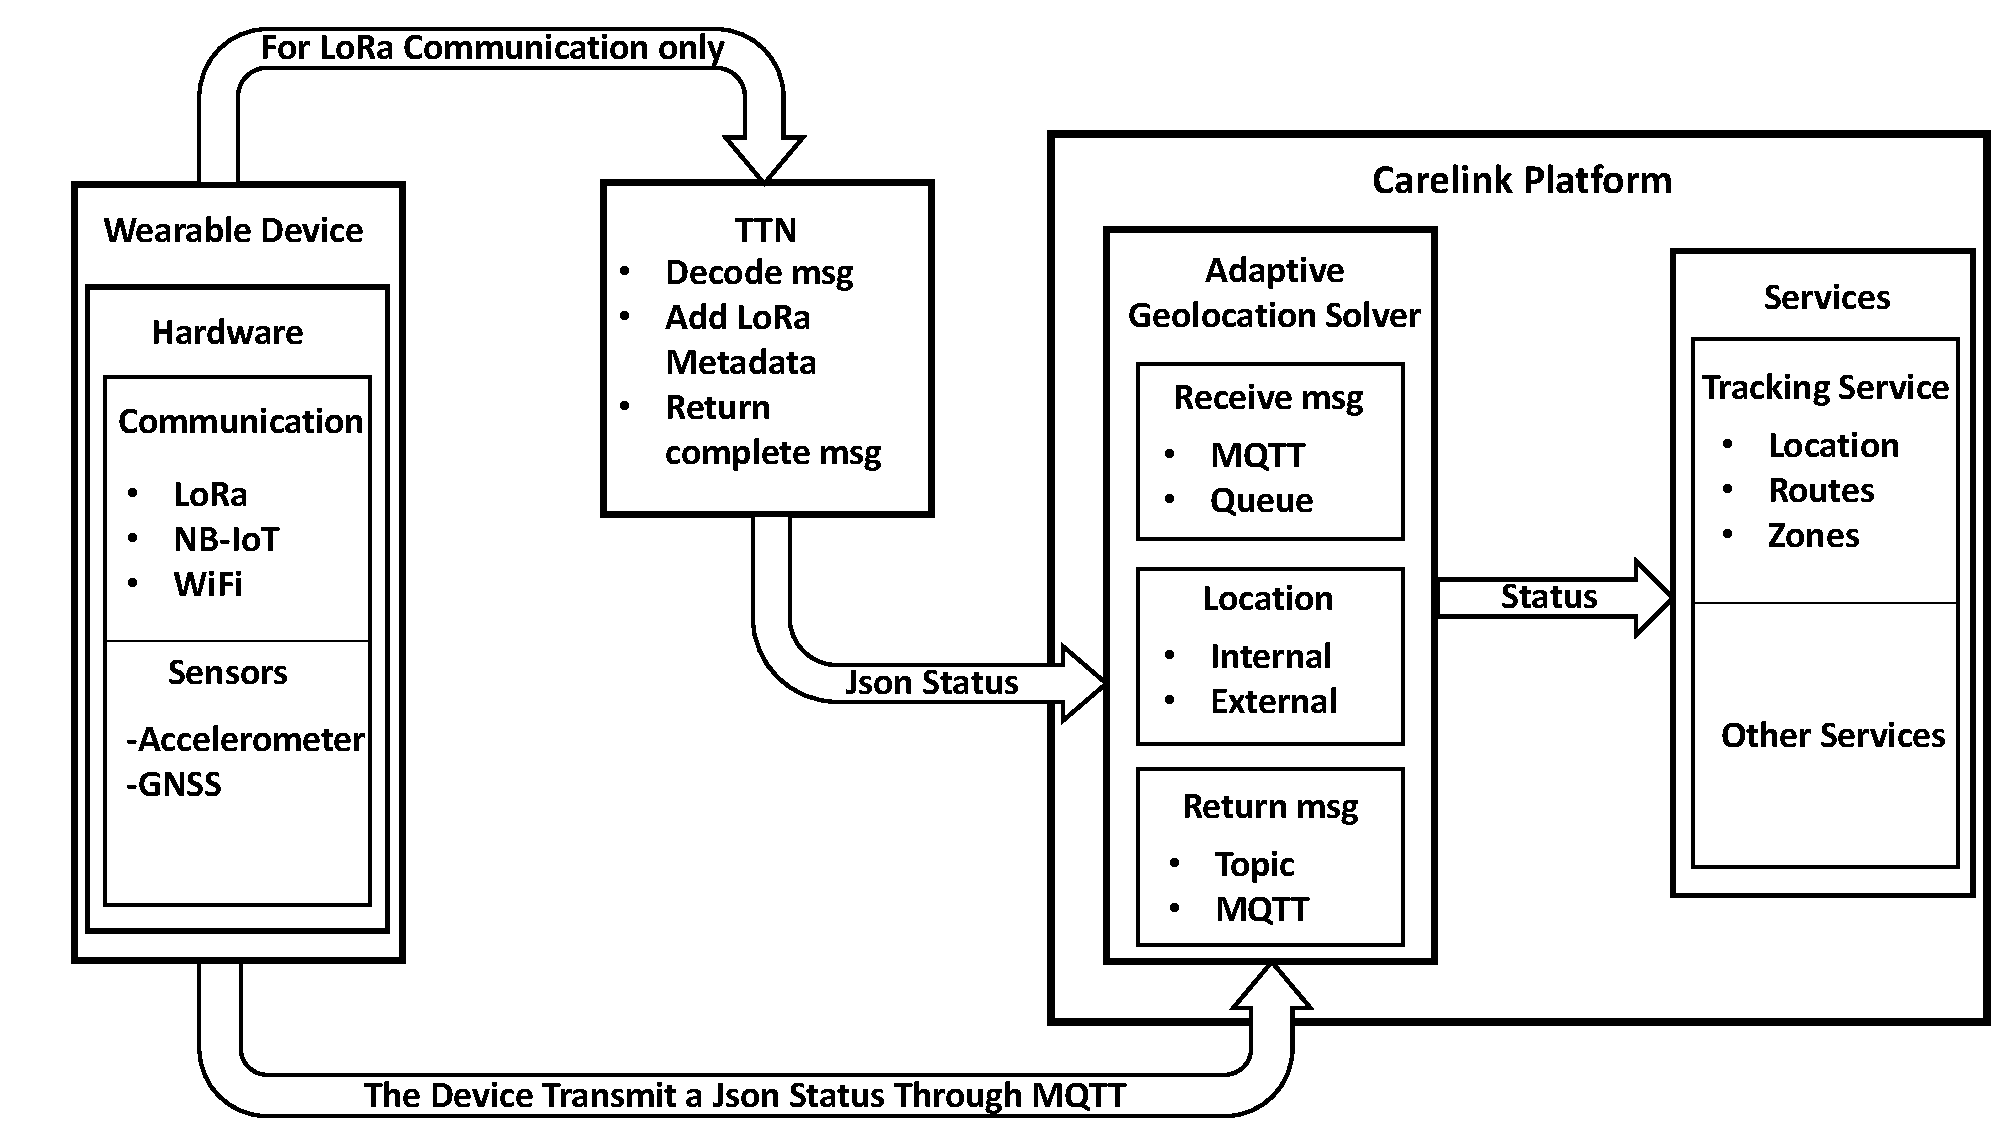
\includegraphics[height=6cm,width=0.9\linewidth]{Chapters/Figures/arch4.pdf}}%
    %}
 
  \caption{Architecture}
  \label{fig:Arch}
\end{figure}


A major part of the system is the communication between the different entities.
These entities will be connected through different protocols and communication standards. The following section explains the protocols used, as well as the more technical part of this work

\section{Wearable Device} % (fold)
\label{sec:Wearrable_Device}
There are two types of wearable devices for the Carelink project, the one represented in~\ref{fig:Insole} as a shoe insole and the other one is the~\ref{fig:Belt_Box} as a belt box. 
These two formats allow different types of utilization, according to the use scenario and user preferences.  
The belt box is designed to be attached to the belt of the user, in a comfortable position.
The shoe insole is intended to replace the existing detachable insole of the shoes and consist of 2 rigid heels and 2 comfort insole fillings. The rigid plastic heel houses the hardware on the right foot insole and a dummy counterweight on the left.
Both types of wearable plastic enclosures have a micro USB connector slot for device charging purposes.
%height=2.9in
\begin{figure}[htbp]
  \centering
  \subcaptionbox{Insole\label{fig:Insole}}%
    {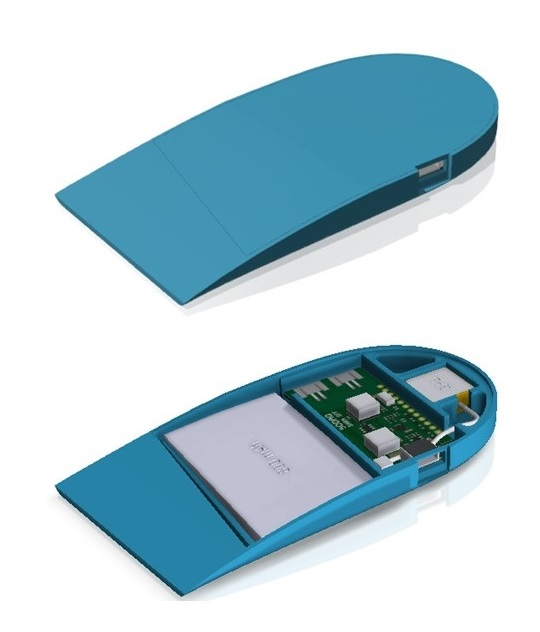
\includegraphics[width=0.45\linewidth]{Chapters/Figures/hardware11.jpg}}%
  \subcaptionbox{Belt Box\label{fig:Belt_Box}}%
    {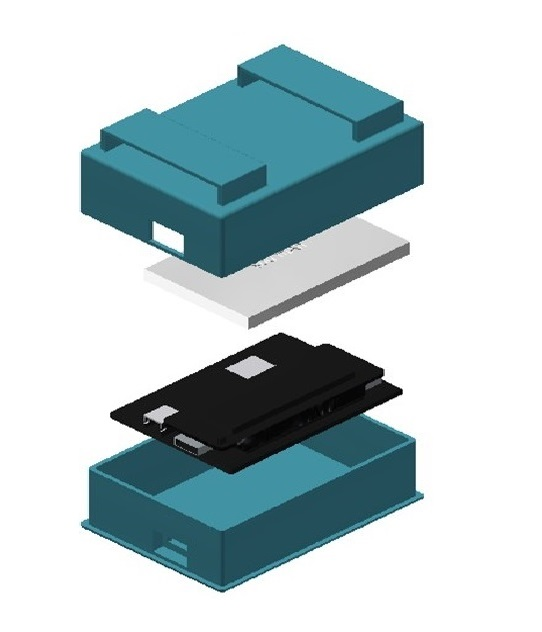
\includegraphics[width=0.4\linewidth]{Chapters/Figures/hardware2.jpg}}%
  \caption{Wearable Devices}
  \label{fig:Wearable_Devices}
\end{figure}


\subsection{Hardware}
\label{susec:Hardware}

In terms of hardware, both of the above wearables offer GPS location tracking and NB-IoT network communication, and they are powered by an 800 mAh LiPo battery. 

The Hardware inside the Insole is a SODAQ SARA R412m presented in the~\nameref{tab:NB-comparison}, where the main advantage is the small form factor, but the problem for this work is that only supports NB-IoT communication.

On the other hand, the belt box was implemented using the FiPy~\cite{Microcontroller2017,Fipy} from Pycom, mounted on PyTrack~\cite{Pytrack} development board both of them represented in Figure~\ref{fig:Fipy_Pytrack}. The FiPy and PyTrack were chosen for a number of practical reasons:
\begin{itemize}
  \item The FiPy is able to run programs written in the Python programming language, allowing for rapid prototyping and development.
  \item The FiPy is capable of having Five networks in one small board(55mm x 20mm x 3.5mm), which is ideal for an Adaptive Geolocation model.
  \item The PyTrack development board contains both an accelerometer and a GNSS module, as well as, providing an easy way of charging and the programming the device.
\end{itemize}
\begin{figure}[htbp]
  \centering
  \subcaptionbox{FiPy~\cite{Fipy}\label{fig:Fipy}}%
    {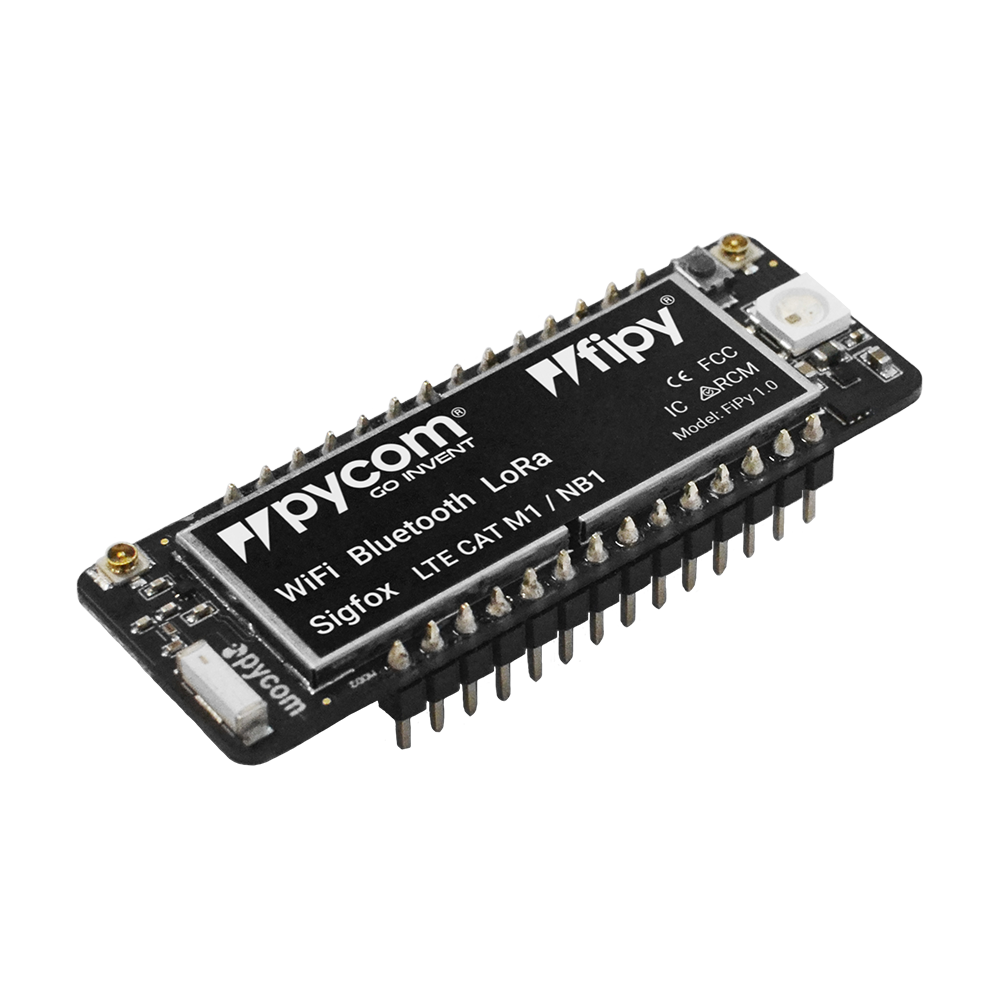
\includegraphics[width=0.33\linewidth]{Chapters/Figures/fipySide.png}}%
  \subcaptionbox{Pytrack~\cite{Pytrack}\label{fig:Pytrack}}%
    {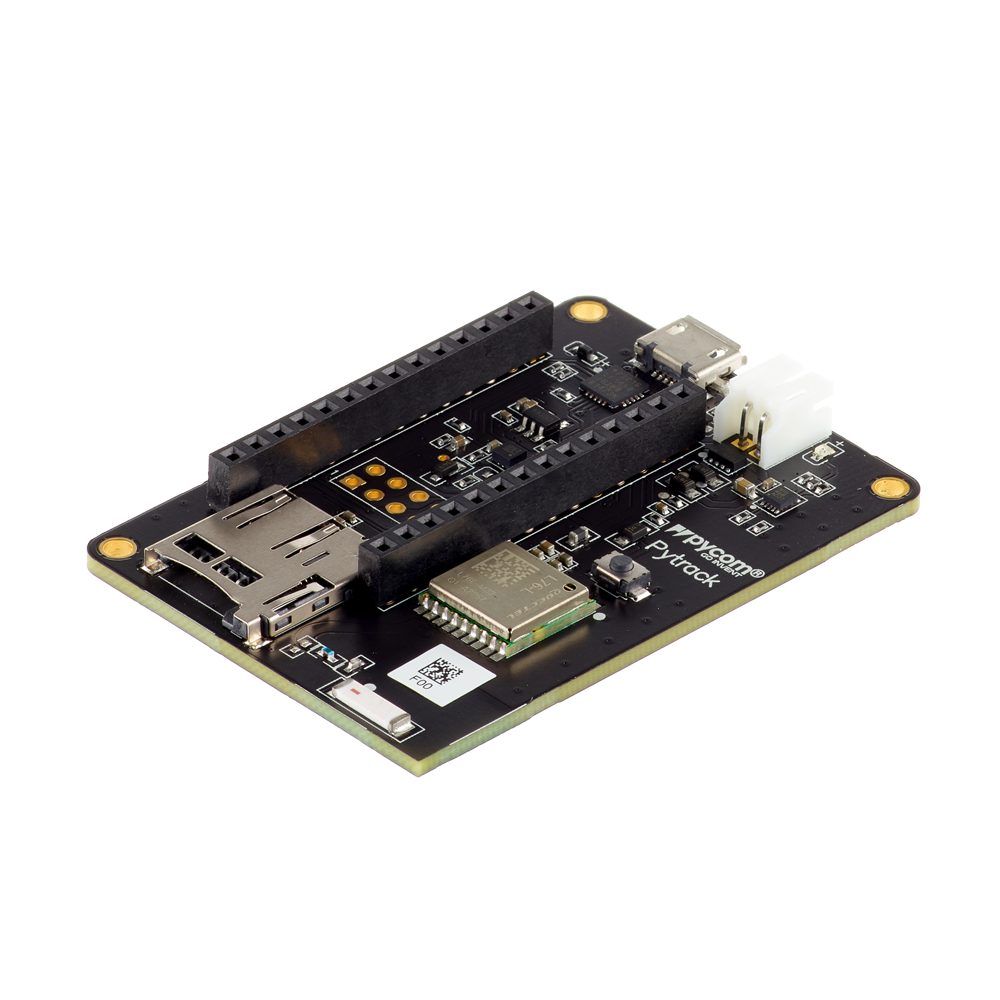
\includegraphics[width=0.33\linewidth]{Chapters/Figures/Website-Product-Shots-Pytrack-Side.png}}%
  \subcaptionbox{Combined~\cite{Pytrack}\label{fig:FipyPytrack}}%
    {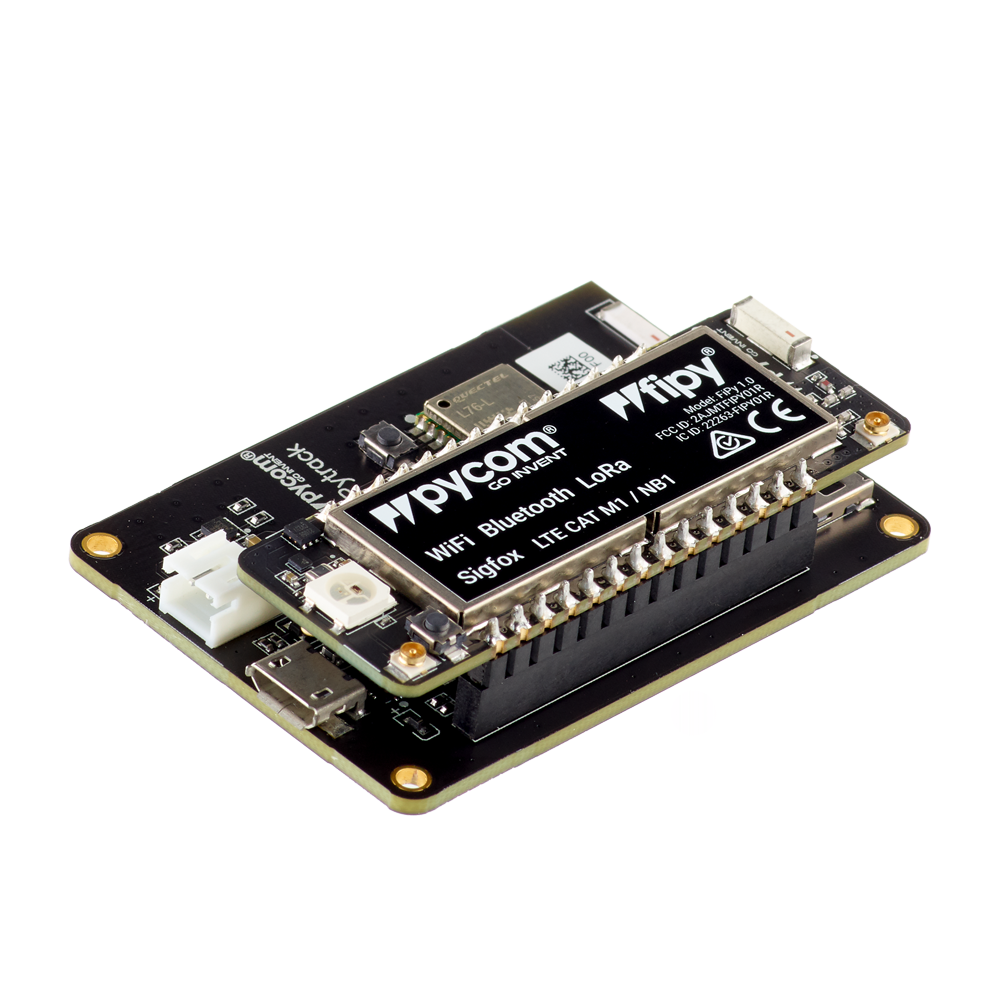
\includegraphics[width=0.33\linewidth]{Chapters/Figures/Website-Product-Shots-Pytrack-FiPy.png}}%
  \caption{Fipy \& Pytrack}
  \label{fig:Fipy_Pytrack}
\end{figure}

The  sensor data from the accelerometer was used  for predicting falls, while the GNSS module provided the location.
The FiPy board includes a Semtech LoRa transceiver SX1276 radio, to which an SMA Tilt Swivel 1/2 Wave Whip Dipole antenna was externally attached for testing, and for the final product a Molex ISM 105262 omnidirectional with 0.4 dBi Peak Gain at 868MHZ. For the WiFi and BLE was used the internal antenna, and for NB-IoT was used a PCB trace antenna. The chipset of the development board is an Espressif ESP32 containing a dual-core Xtensa 32–bit LX6 capable of up to 600 DMIPS, and an extra ULP–coprocessor that can monitor GPIOs, the ADC channels and control most of the internal peripherals during deep–sleep mode while only consuming 25uA.
%\begin{figure}[htbp]
%  \centering
%    {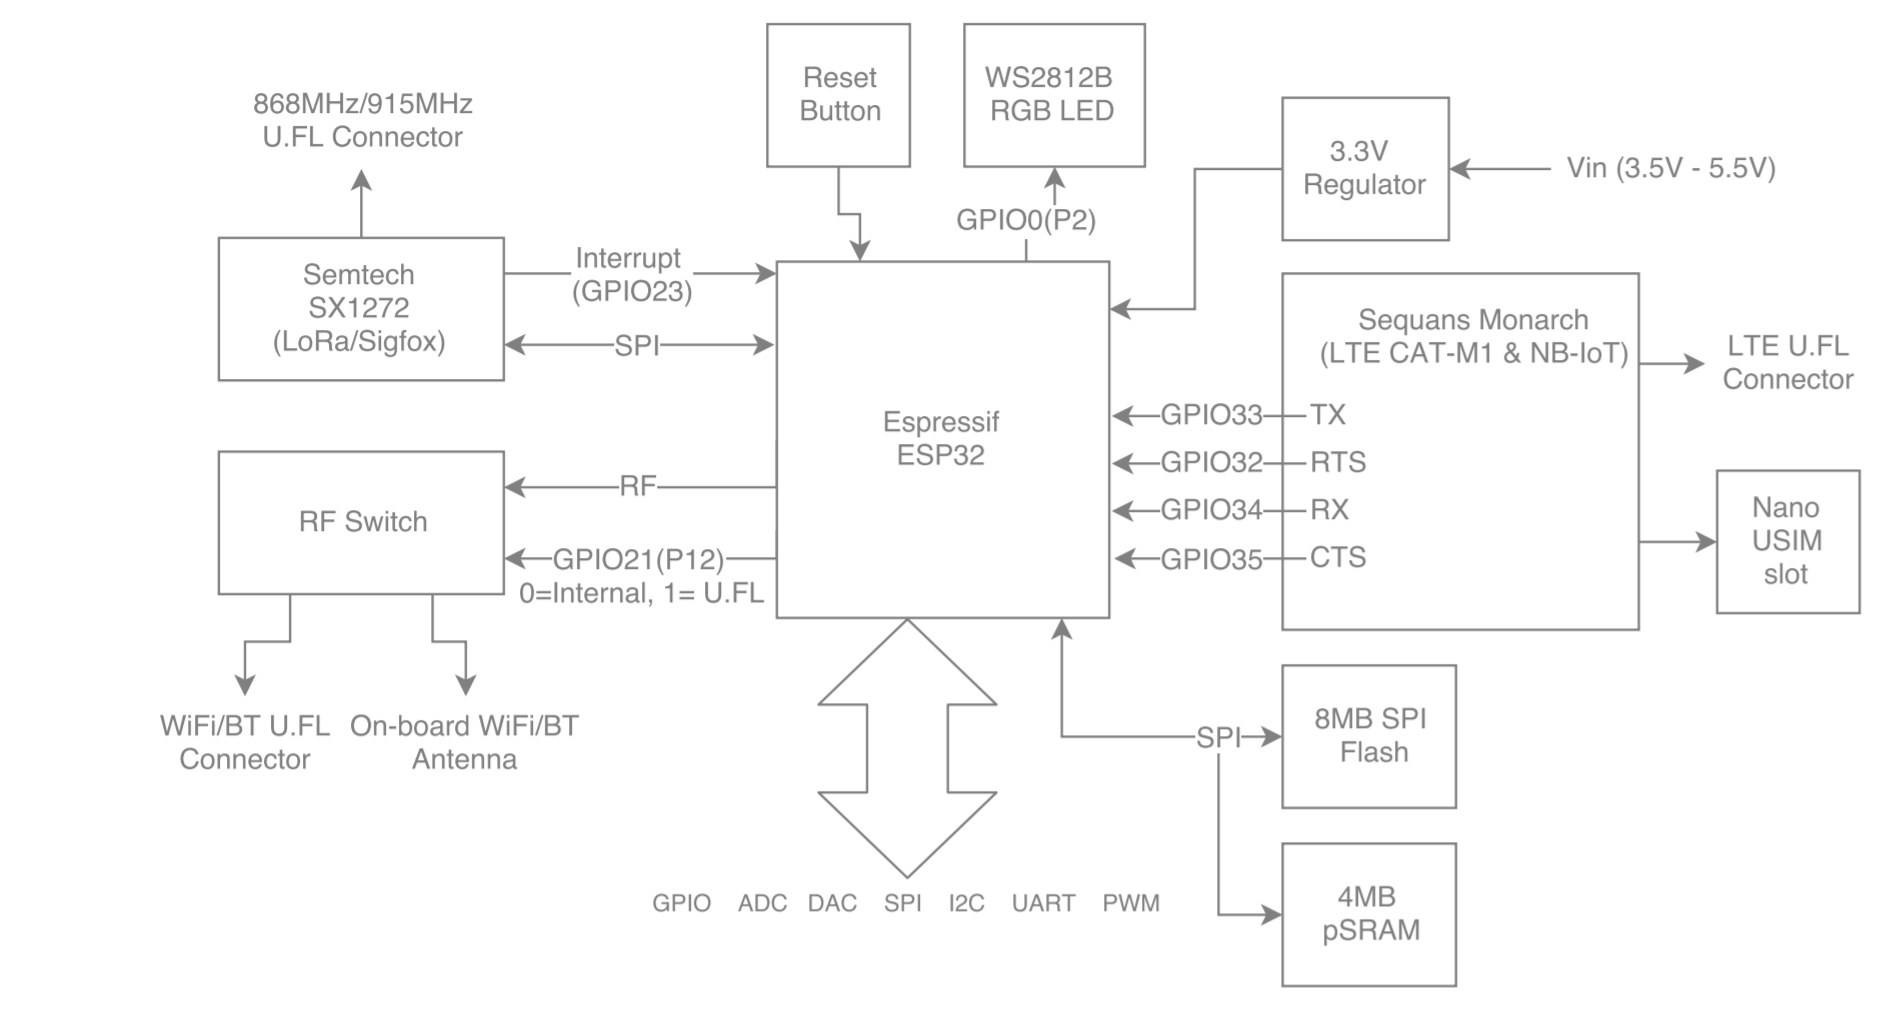
\includegraphics[width=0.85\linewidth]{Chapters/Figures/blockdiagram.PNG}}%
%  \caption{FiPy Block Diagram}
%  \label{fig:Block_diagram}
%\end{figure}

\subsection{Operation}
\label{susec:Operation}
The Device operation loop is represented in diagram~\ref{fig:Main_Op} below. Where first the device is power up, then proceeds to initial verification's and setup, the next block that can be seen in more detail in  figure~\ref{fig:Connect}, is the connect. Following this operation exists two options either the device is not connected, and enters in backup mode, or is connected and starts the operation of getting the energy profile, pull sensor data and getting the location. After this enters in sleep mode for saving energy and then the cycle starts again.

\begin{figure}[htbp]
  \centering
  
    {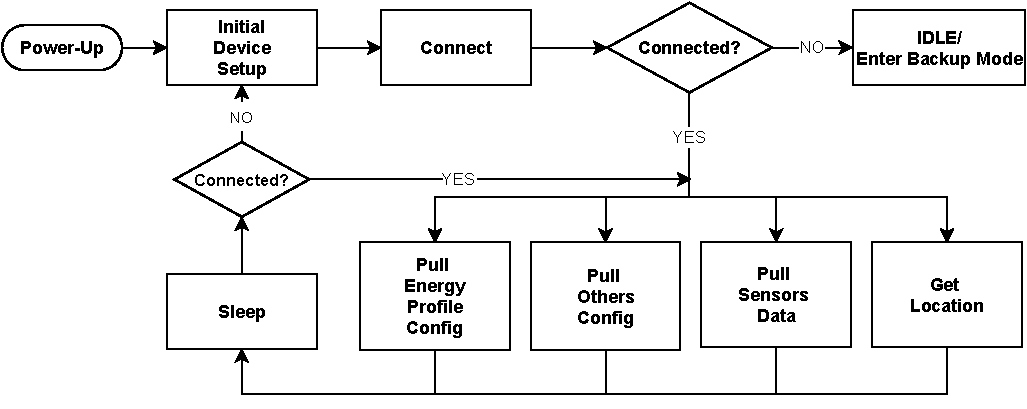
\includegraphics[width=0.8\linewidth]{Chapters/Figures/Main.pdf}}%
 
  \caption{Main Operation}
  \label{fig:Main_Op}
\end{figure}

Inside the Connect block, is a state machine, as it is possible to observer bellow in Figure~\ref{fig:Connect}. This Block is responsible for doing the Adaptive selection of the transmission method, assuring the high availability needed for this work. The selection option for the transmission may vary from the two LPWAN, NB-IoT or LoRa, and WiFi. This development board also support BLE, that will be just for sniffing and collect location, not has transmission method, and Sigfox. That is also an LPWAN, but due to the maximum message size, and the daily message limit, is not suitable for the use case, where this work is inserted.

\begin{figure}[htbp]
  \centering
  
    {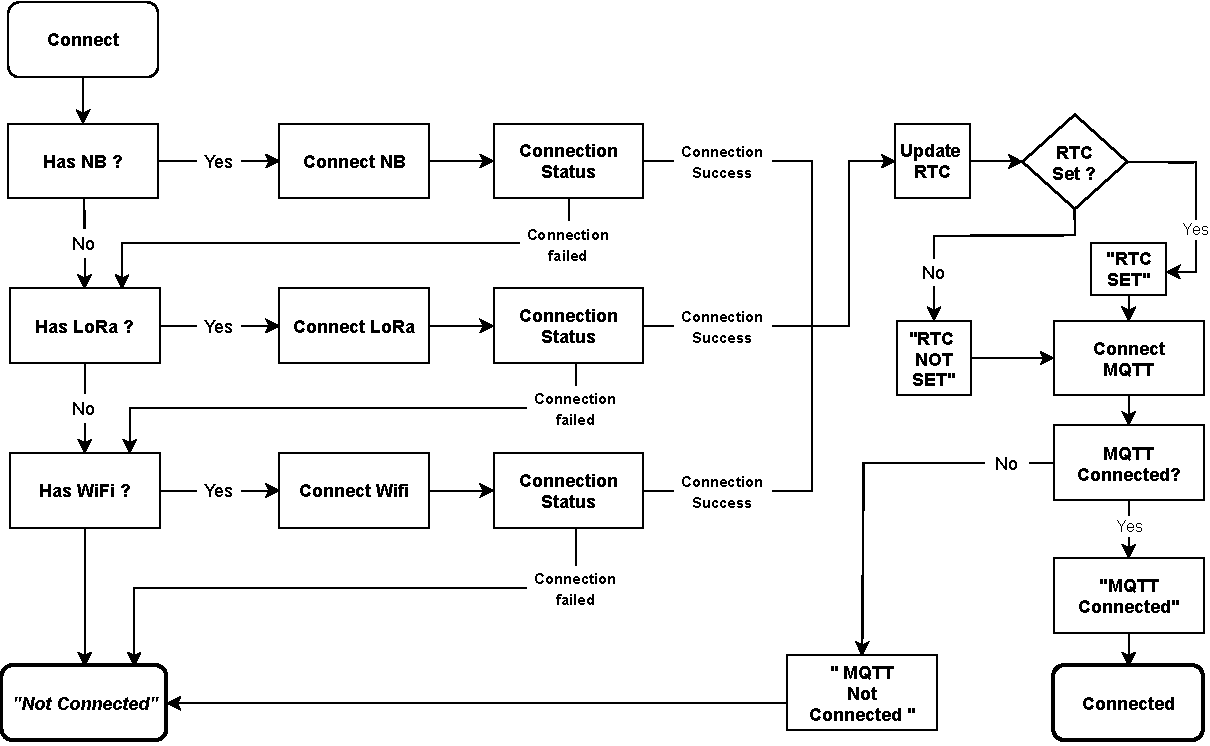
\includegraphics[width=\linewidth]{Chapters/Figures/Connect.pdf}}%
 
  \caption{Connect}
  \label{fig:Connect}
\end{figure}

As it is possible to observe in the figure above, the first block is NB-IoT, then LoRa and in the end WiFi, this is the usual operation but can be changed according to the energy profile. This order was defined not because of battery or range but coverage. First NB-IoT should have higher coverage, then if this one fails there is  LoRa with the possibility of using community gateways, or even create a private ad-hoc network, the last one WiFi is only used in case none of the others work.



Following the previous diagram the next figure~\ref{fig:ConnectLoRa}, represents how the connect LoRa block works. First, one of the classes that were represented by the previous figure~\ref{fig:lora_classes}, is set followed by the adding channels. After that, there is the activation, the selected mode for security reasons~\ref{fig:lora_security}, was~\gls{OTAA}. When this activation is finished, and there is a gateway listening and accepting the join request, the LoRa transmission starts. The other method for activation is~\gls{ABP}.

Connect LoRa is, in fact, a python class that was created and this diagram represents the \verb| __init__ |method, after creating the Lora object, exists a thread running for doing the LoRa transmission.\newline
\begin{figure}[htbp]
  \centering
  
    {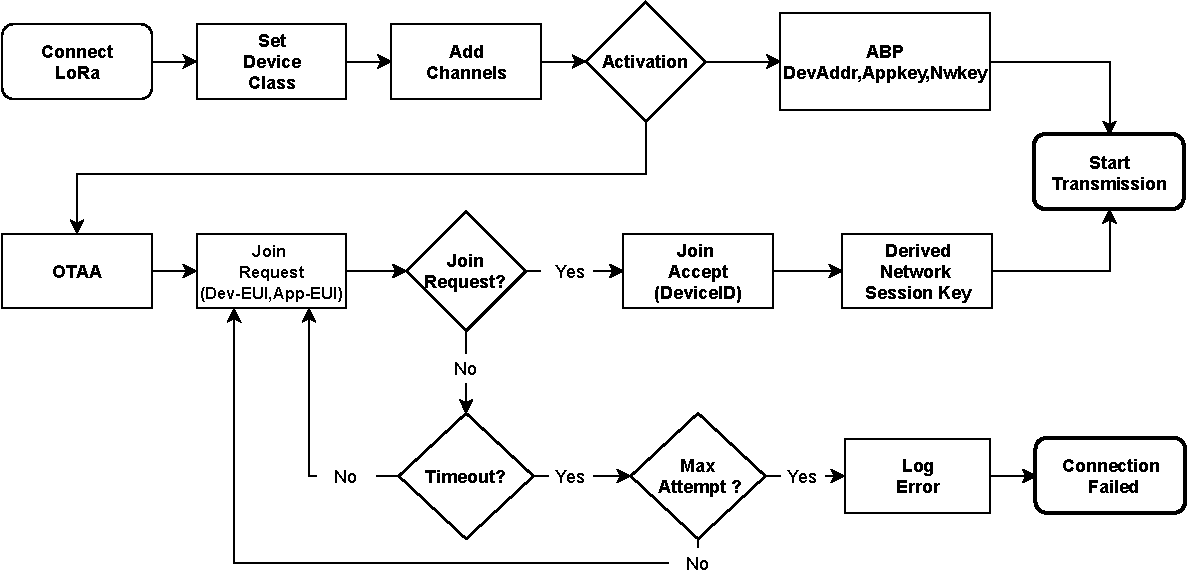
\includegraphics[height=7cm,width=\linewidth]{Chapters/Figures/ConnectLoRa.pdf}}%
 
  \caption{Connect LoRa}
  \label{fig:ConnectLoRa}
\end{figure}

On the device, the work done regarding communication consists, in the use of~\gls{MQTT} between the device and the model. When the transmission method used is LoRa there is the need for an extra layer of "translation" as explained in the next section~\nameref{sec:server}.

\newpage
The next Figures represents the piece of code, that is executed inside the "Start Transmission"  block. In this function all of the values of JSON Status~\ref{fig:JSON_Status}, are assigned with the default value in all of them is 0, even for a timestamp that is the begin of the UNIX time. This is going to be applicable in later stages for debugging and make decisions, in case these values do not change.
\begin{figure}[htbp]
  \centering
  
    {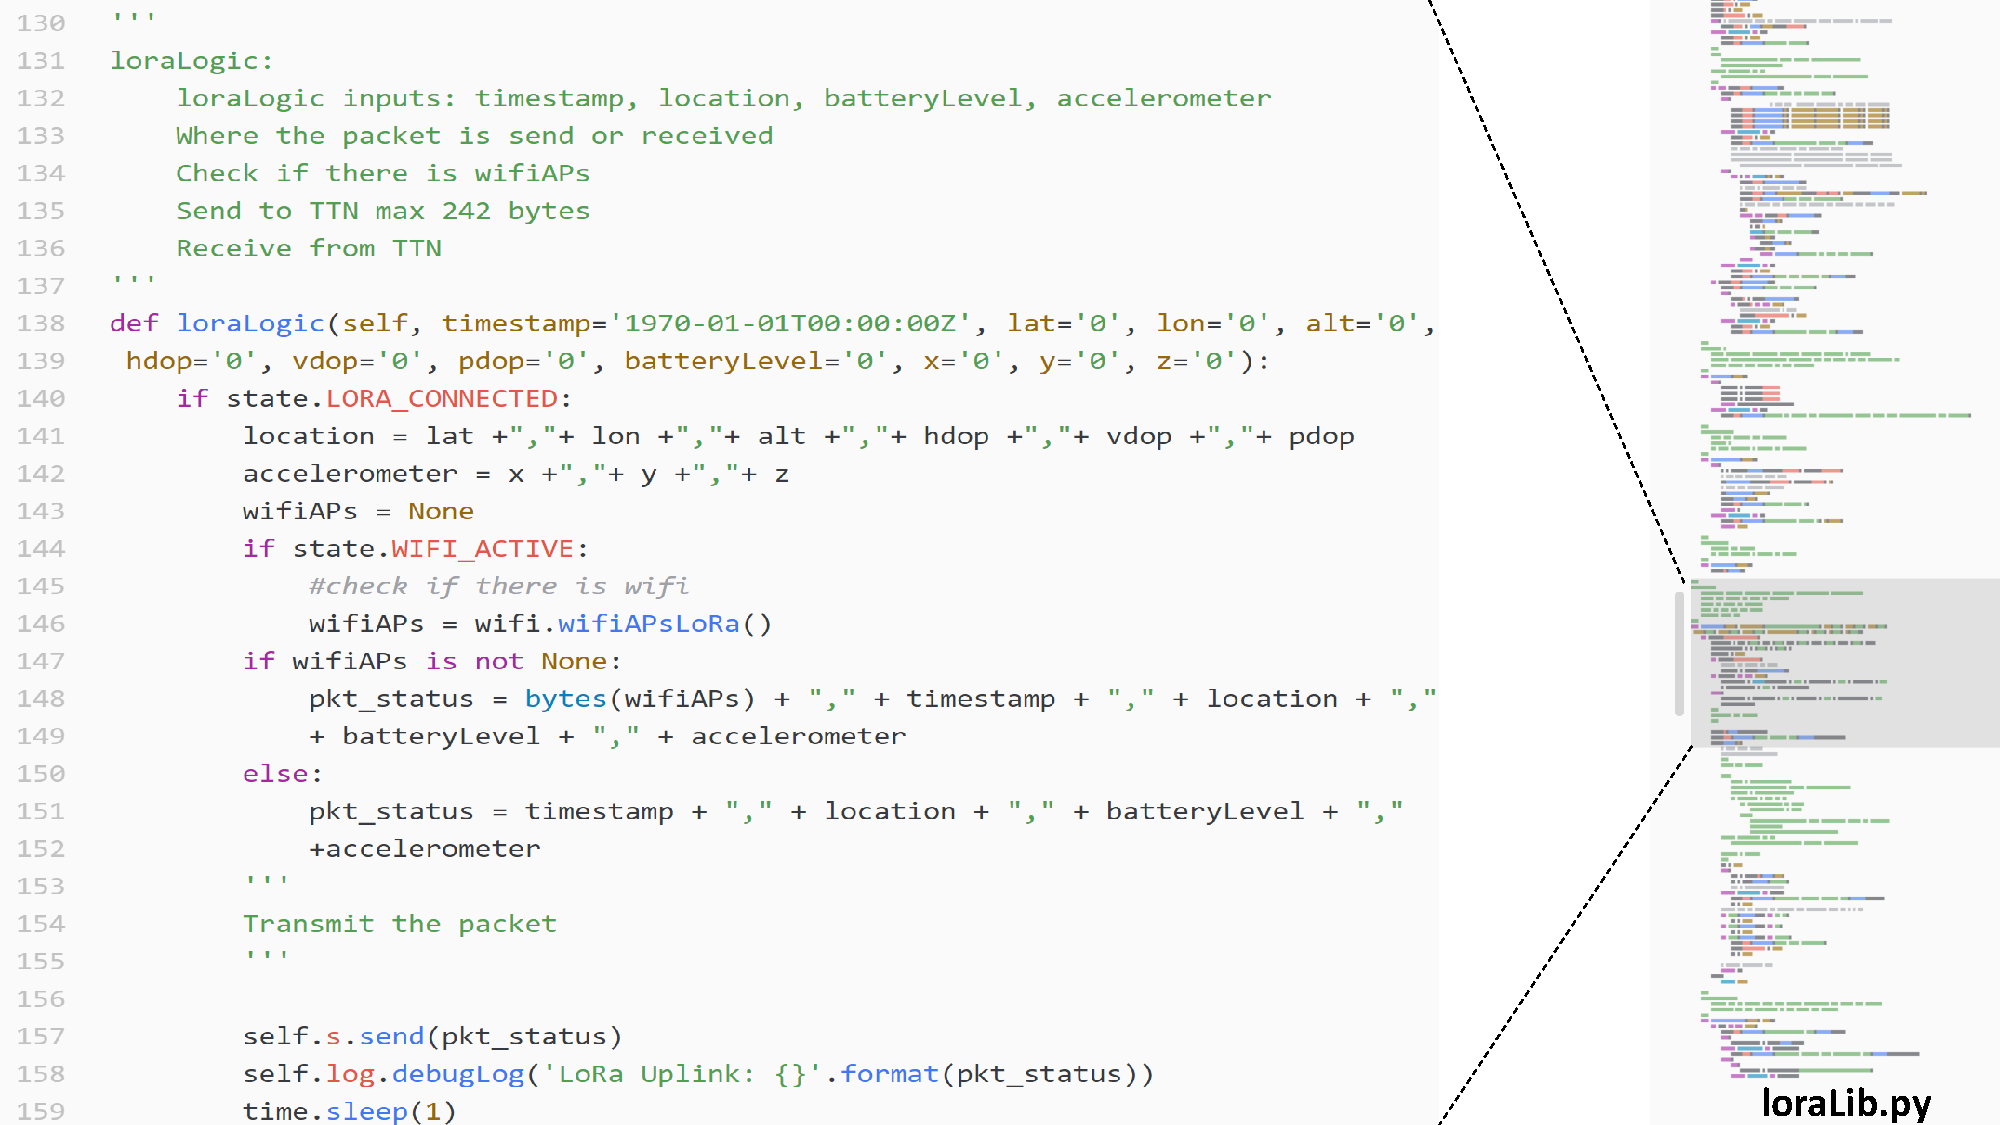
\includegraphics[width=0.9\linewidth]{Chapters/Figures/loralib.pdf}}%
 
  \caption{LoRa Transmission from loraLib.py~\cite{githubcode}}
  \label{fig:LoRa_Transmit}
\end{figure}

The last thing in the Hardware side, for the Adaptive Geolocation model, is the ability of the device, sensing the surrounding environments this can be achieved for example through WiFi sniffing. With the gathering of this data (BSSID and RSSI), as represented in the following figure~\ref{fig:WifiAps}, is possible to estimate the location of the device using assisted location. 

\begin{figure}[htbp]
  \centering
  
    {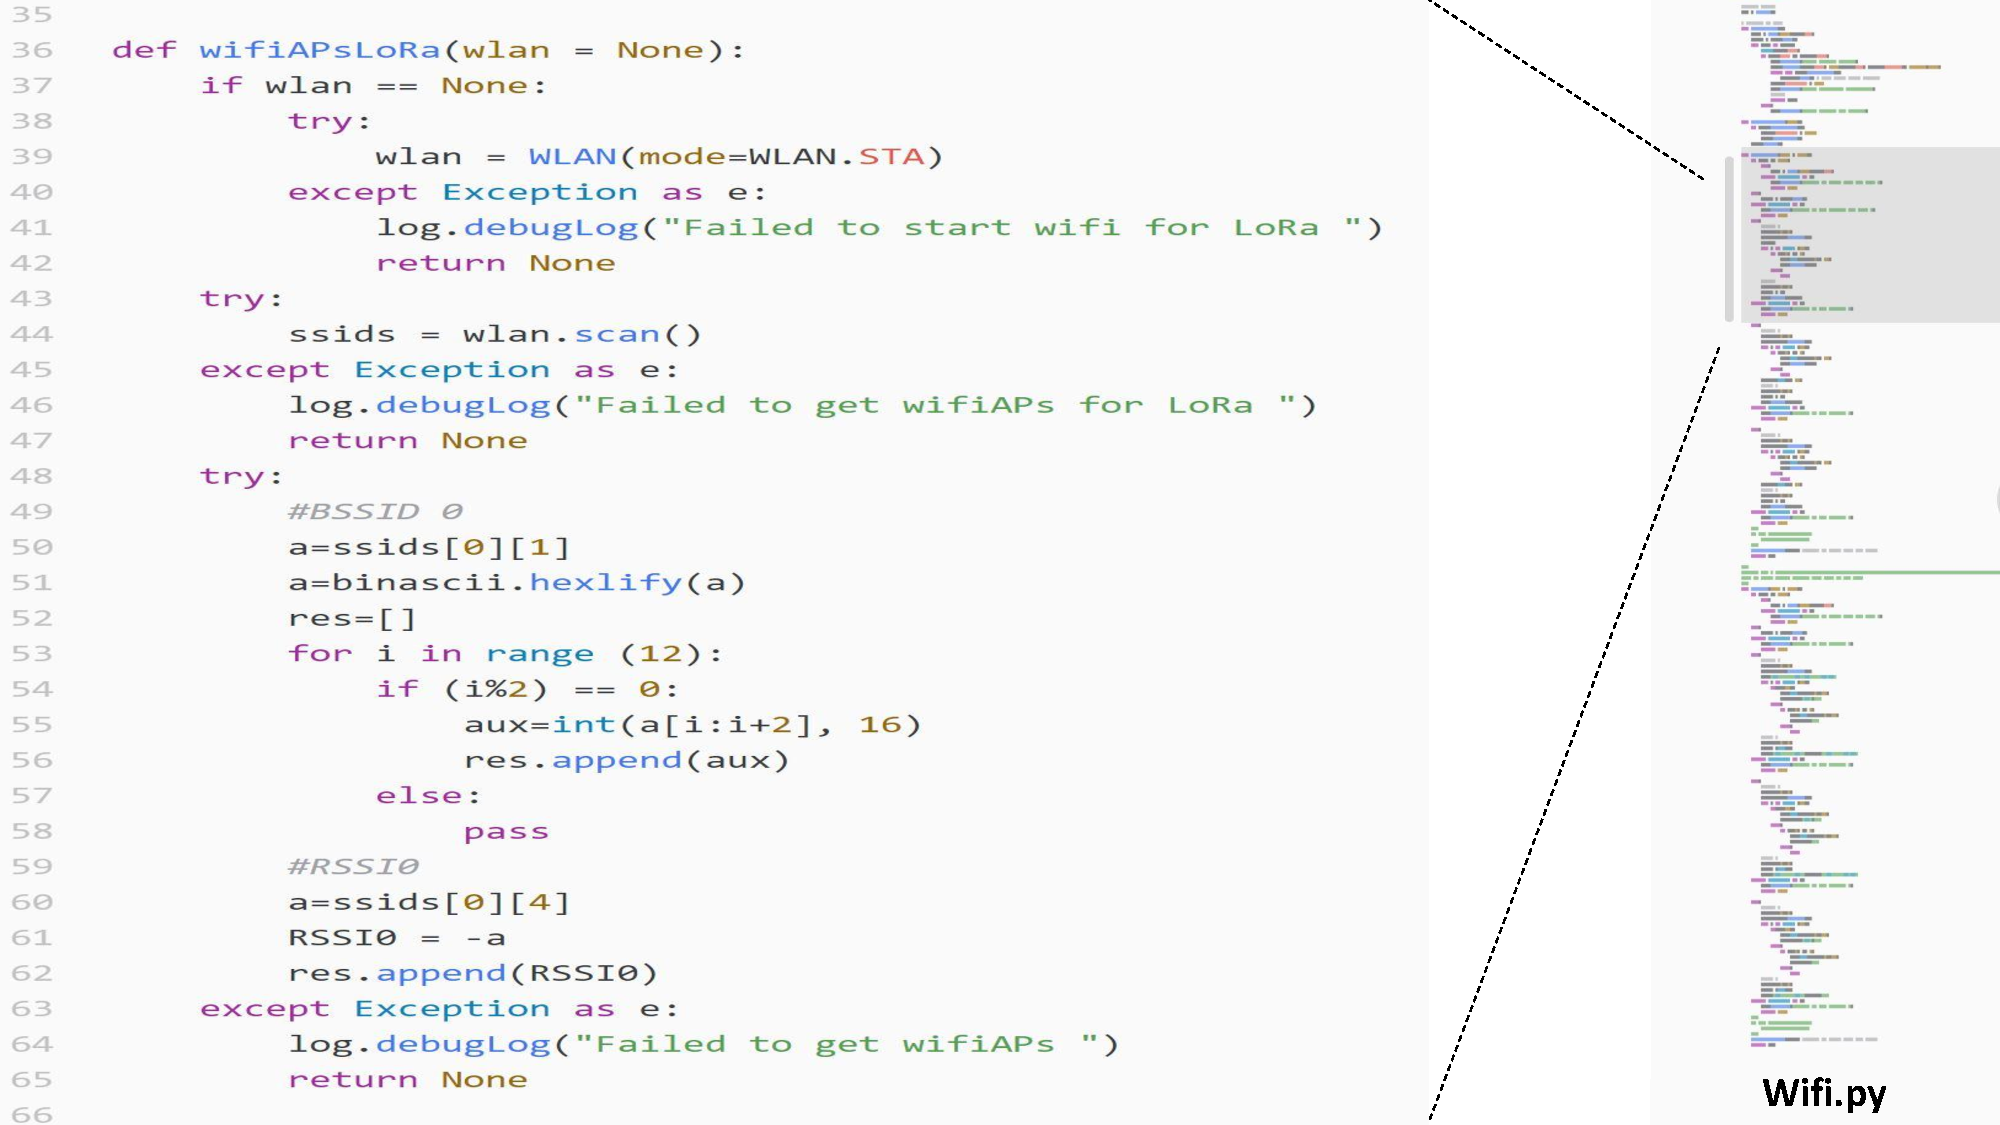
\includegraphics[width=0.9\linewidth]{Chapters/Figures/wifi.pdf}}%
 
  \caption{WiFi APs Code from wifi.py~\cite{githubcode}}
  \label{fig:WifiAps}
\end{figure}

The two previous images~\ref{fig:WifiAps} and ~\ref{fig:LoRa_Transmit}, are pieces of code, retrieved from two source files, where the author had contributed, this two files combined with other 18 are which defined the working principle of the device and can all be found at~\cite{githubcode}. 



%\subsection{Communication}

%\label{susec:Communication}

%On the device the work done regarding communication consists, in the use of~\gls{MQTT} between the device and the model. When the transmission method used is LoRa there is the need for an extra layer of "translation" that where the next section comes in.  


\section{LoRa Network Server} % (fold)
\label{sec:server}
\subsection{TTN} % (fold)
\label{sec:TTN}
The Things Network (TTN)~\cite{TTN} acts as the network server, and is responsible for providing a bridge, between LoRa communication and the internet. Also when TTN receives the information, a decoder function that is in appendix~\ref{app:TTN_decoder} is used, for converting the received message payload to the adequate data format.
Moreover, still in the TTN server, the devices are registered in the right application, and the LoRa cloud~\gls{API} integration is used. This~\gls{API} will calculate the current location of the device based on the metadata present in the uplink messages. In the end, TTN will send the result message through MQTT to the Adaptive Geolocation Model.

The next Figure~\ref{fig:TTN_Console}, shows the TTN console for the application. In this console is possible to observe the metadata of the message,  with information about the gateways, as well as, the estimated last location of the device, is also possible to observe the \emph{Fields}, where the decode JSON Status is represented.

\begin{figure}[htbp]
  \centering
  
    {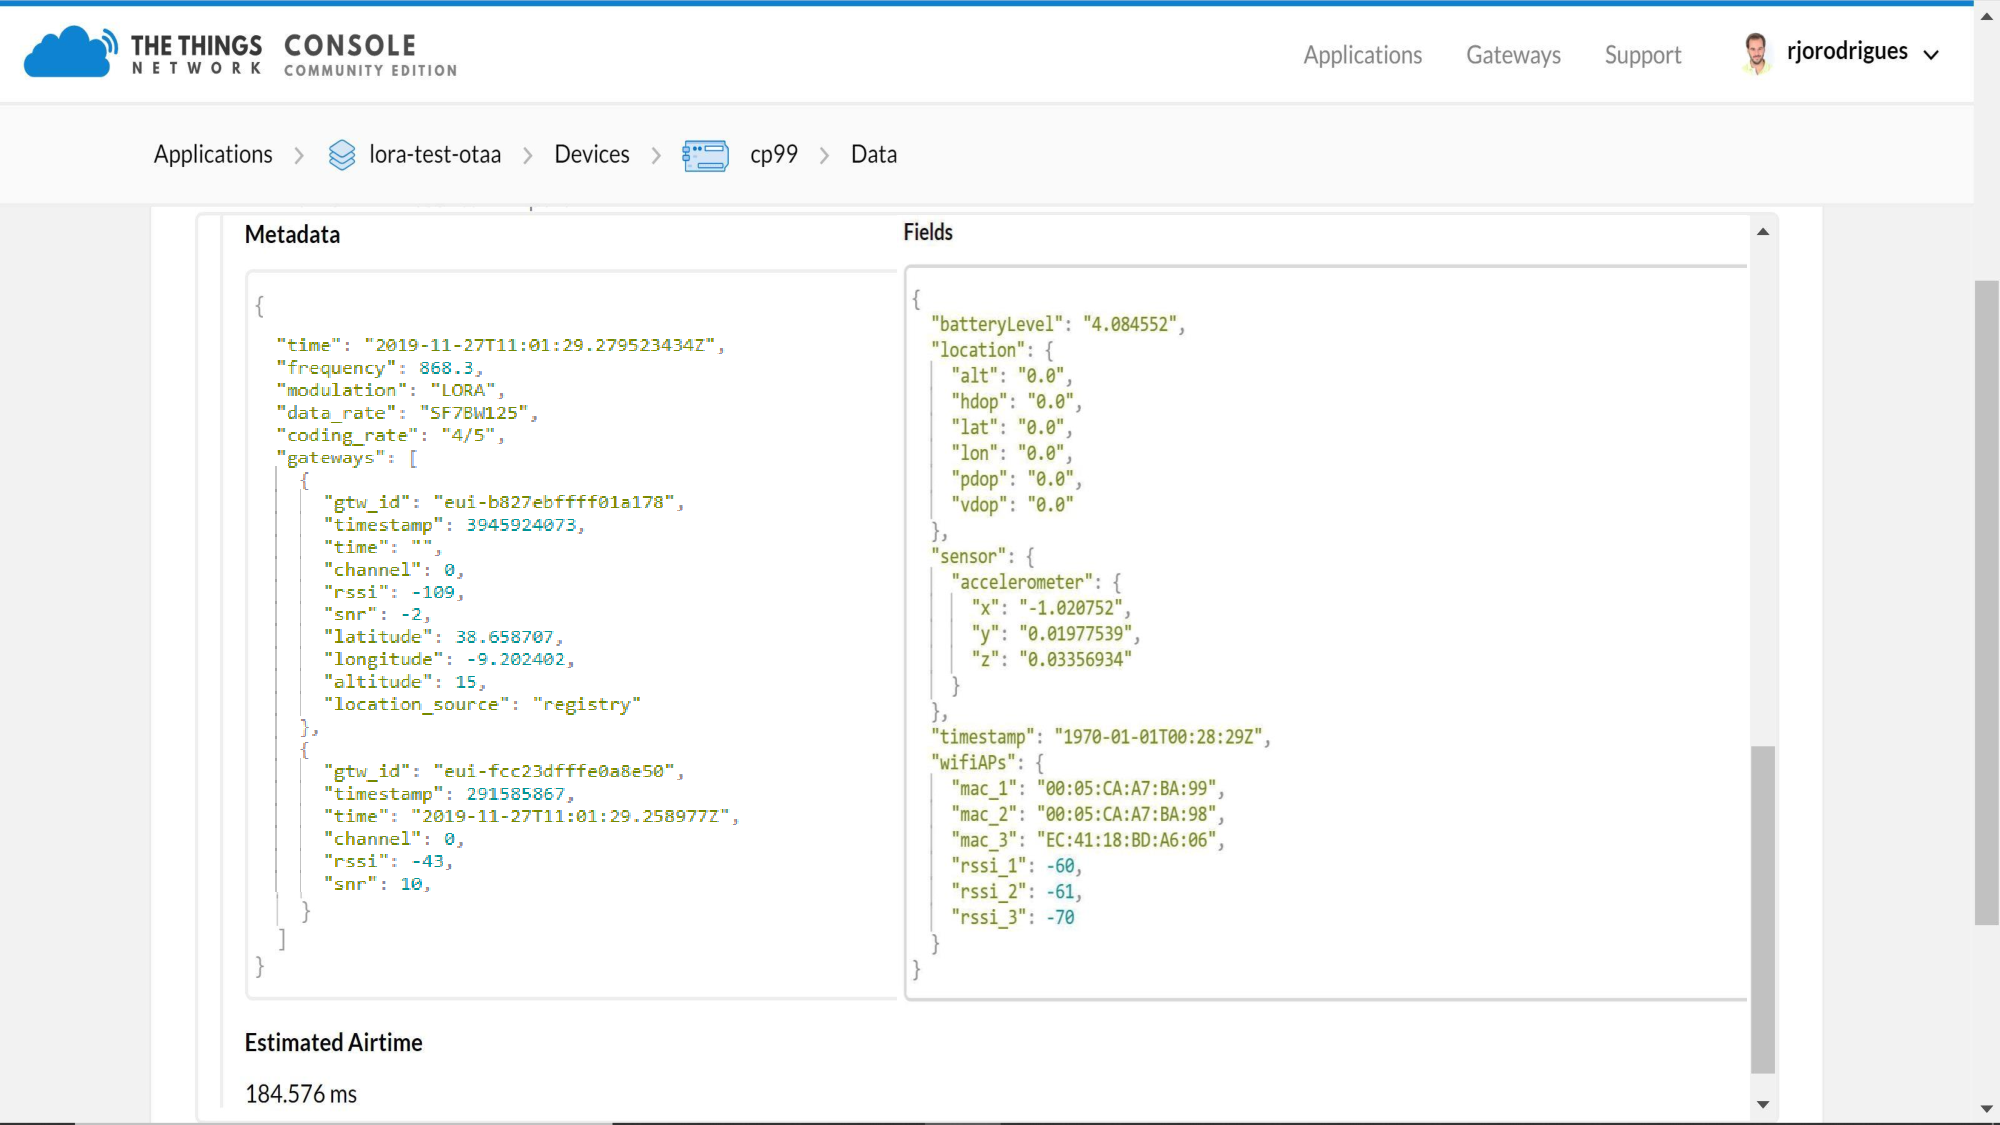
\includegraphics[height=9cm,width=\linewidth]{Chapters/Figures/ttn.pdf}}
 
  \caption{TTN Console}
  \label{fig:TTN_Console}
\end{figure}

For this work, TTN was selected because it was the one with better community support, documentation, and fulfilled the requirements for the use case in study. There is other alternatives for TTN such as  loriot~\cite{Loriot}, thingsboard~\cite{ThingsBoard}, Mbed OS~\cite{Mbed} and Mozilla IoT~\cite{Mozilla}. 


% subsection ttn (end)
\newpage

\section{Adaptive Geolocation Services} % (fold)
\label{sec:Adaptive Geolocation}
For the presented work, to achieve the adaptive Geolocation, was developed and implemented a model called "Adaptive Geolocation Solver". This model is responsible for receiving the data through~\gls{MQTT} from the different communication methods, do the calculation for the best geolocation, and return a~\gls{JSON} called \emph{status} through~\gls{MQTT} to the Carelink~\cite{carelink} platform.
% subsection nodered_sota (end)
\subsection{Node-red} % (fold)
\label{sec:nodered_sota}
%ver secc vertical
The platform chosen by the author for the development of the Adaptive Geolocation Solver, was Node-Red~\cite{Node}.
Node-RED is  Low-code programming, for event-driven applications, it uses development tool for visual programming, was initially developed by IBM, with the intention of wiring together devices, APIs and other online services that were part of the IoT.
Node-RED uses a web browser-based flow editor, that can be used to write JavaScript functions. The run-time is built on top of Node.js. The flows created in Node-RED can be saved using JSON. In 2016, Node-RED was contributed by IBM  to JS Foundation  as an open source project.
The instructions need to replicate this work are in  Appendix~\ref{app:nodered}, and the complete guide can be seen in~\cite{githubnodered}. Although the six main modules will be described below.

\begin{itemize}
   \item \textbf{LoRa Uplink} \\
   As it was introduced in the previous chapter~\ref{cha:Adaptive_Geolocation}, the "LoRa Uplink" module is intended to be used for LoRa Uplink transmissions. Its operation can be seen in figure~\ref{fig:LoRa_Uplink}.
\begin{figure}[htbp]
  \centering
  
    {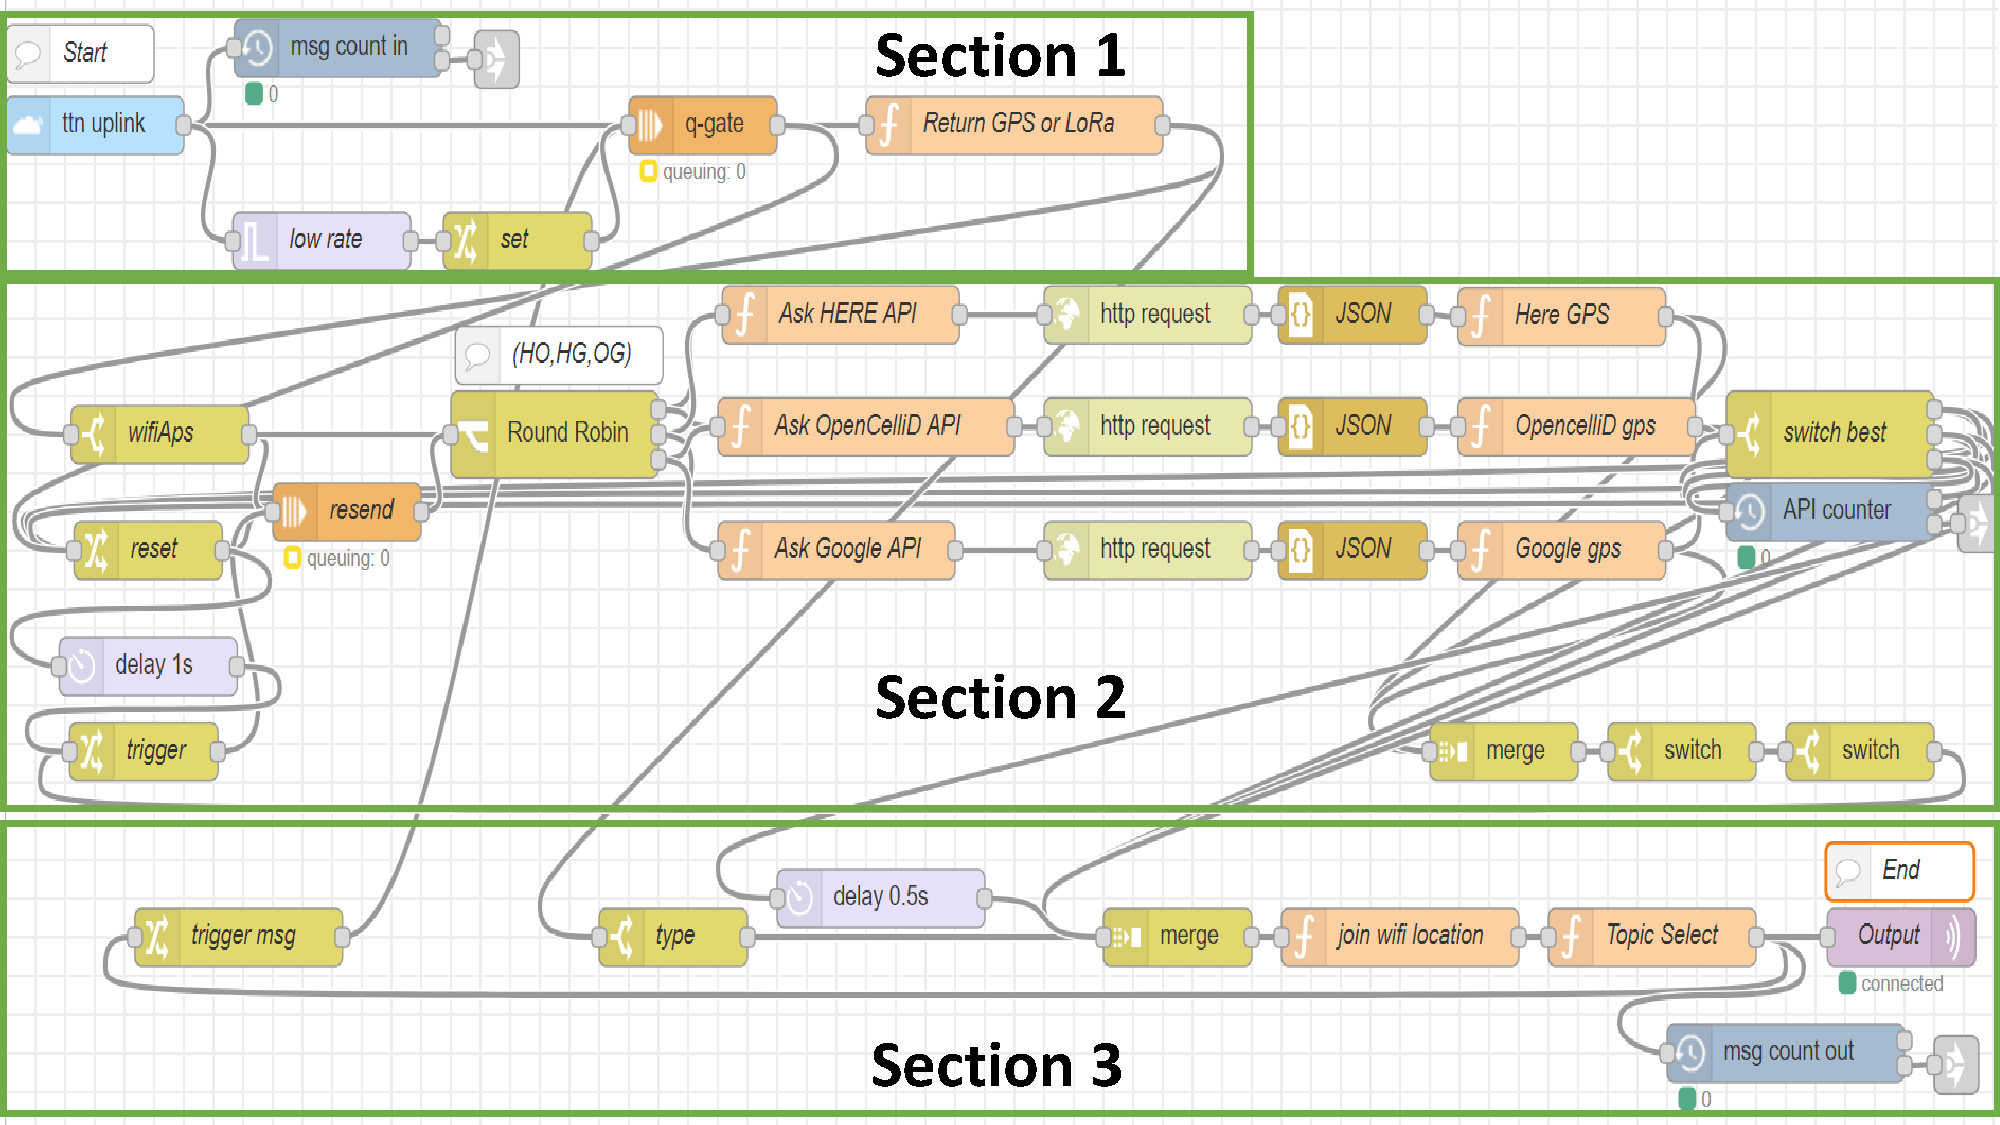
\includegraphics[height=9.3cm,width=0.9\linewidth]{Chapters/Figures/LoRaUplinkFlow.pdf}}
 
  \caption{LoRa Uplink Flow}
  \label{fig:LoRa_Uplink}
\end{figure}
 
As it is possible to observe in the previous figure~\ref{fig:LoRa_Uplink}, the LoRa Uplink module is divided into three sections. In order to better understated its implementation the sections will be described below.

\begin{itemize}
  \item Section 1\\
    In section 1 the model, receives an input message from the TTN, as explained in the~\ref{sec:server}, and this message is stored in a queue with a gate, this queue gate can be trigger activated, which means that a message is only released when the last message was processed. This received message serves as input for monitor counter, and for the LoRa Downlink module, for later use. After the queue is the first function where the message is analysed. If the message contains valid GPS data, the next section is section 3. If there is no GPS data but Wi-Fi data is available the next section is section 2. 
   
\end{itemize}

\begin{itemize}
  \item Section 2\\
    At section 2 the Wi-Fi data is first analysed, and then is sent to the load balancer, at the same time is stored in a second queue. The load balancer distributes the messages through the 3 APIs, following the equation presented in~\ref{eq:loadbalancer}. If the two chosen APIs, failed to delivery the location, the gate is activated, and the message is resent to another API. If the location is successfully received the queue is cleared, and the location with the best accuracy is sent to section 3.

\end{itemize}

\begin{itemize}
  \item Section 3\\
  In this last section the received information from section 1 and 2 is analysed. The first function ensures that the previous information is not null, then the original information is merged  with the information from section 2. After that, the correct topic is selected  the final information is sent, to the MQTT broker of the Carelink platform. At the end of the function responsible for the selection of the correct topic, is the monitor counter, and a connection to the trigger of the first queue, in order to release the next message.

\end{itemize}

\end{itemize}


\begin{itemize}
   \item \textbf{LoRa Downlink} \\
   The Carelink platform is capable of  communicating directly with devices, through MQTT, but this is not possible directly using LoRa as explained earlier in section~\ref{cha:Implementation}, so this module acts as a middle layer for the communication. This module is represented in figure~\ref{fig:LoRa_Downlink}, on the left side of this figure, are the subscribed MQTT topics. In the bottom of the figure is the input message from the LoRa Uplink module, which was used to send a "ping" message to the device, this was used for knowing that the device was still alive. The other solution was to use Uplink confirmations, but this was less power efficient. The workflow behind this module is the following: First, subscribe to the MQTT topics, then convert the information to base64, select the correct node and send to TTN.\newline\newline\newline\newline
   
     \begin{figure}[htbp]
      \centering
      
        {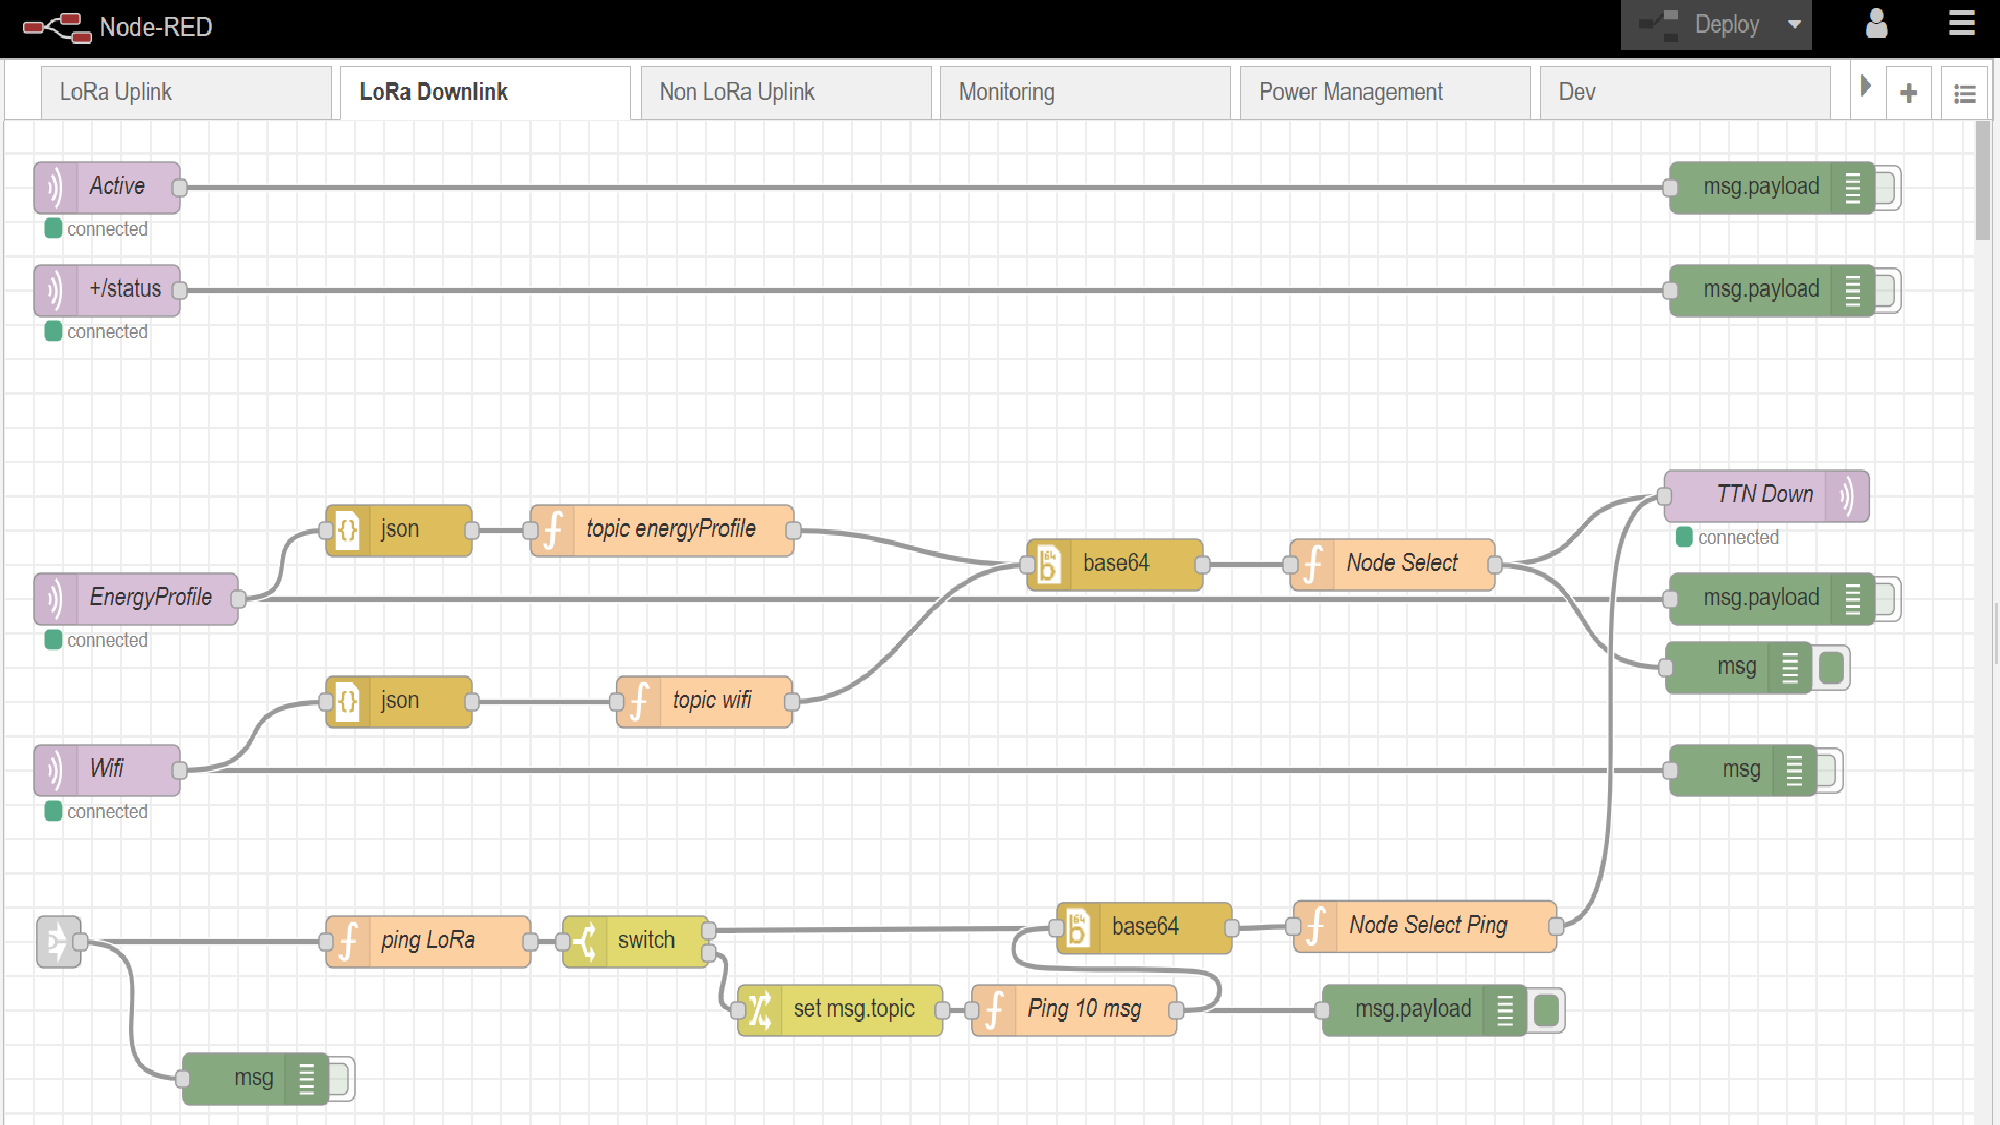
\includegraphics[height=9.5cm,width=0.9\linewidth]{Chapters/Figures/LoRaDown.pdf}}
     
      \caption{LoRa Downlink Flow}
      \label{fig:LoRa_Downlink}
    \end{figure}
\end{itemize}


\begin{itemize}
   \item \textbf{Power Management}\\
   This module is  responsible for the power management of the devices, and it is used mainly in the last two functional stages ("Advanced"  and "Smart"). The module is represented in  figure~\ref{fig:Power_Management}. The working principle is the following first on the left side of the figure, the status topic is subscribed. Then the message is converted to JSON, and is filtered only the messages from Pycom devices. The message is analysed and the battery level is checked. If the battery level is valid, the remaining battery is calculated, as well as, the percentage of the total capacity, for example, "CP20" 10 hours 90\%. Then based on this information the active components and the sample rate of them are adjusted. For the later stage, this module could take into account if the device is paired  with carer smartphone, by checking the "accompanied" flag of the status message, and by subscribing "zones" topic check where the device is working, being the possibilities the following: home, regular, dangerous. This was defined by Jorge in~\cite{githuMQTT}, but not implemented in this module.
    \begin{figure}[htbp]
      \centering
      
        {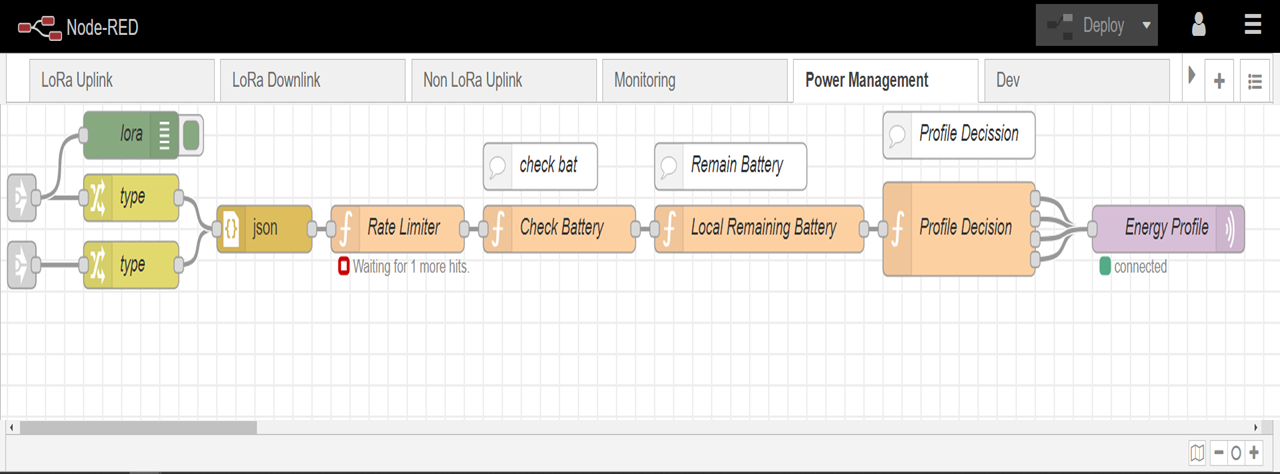
\includegraphics[height=4cm,width=0.9\linewidth]{Chapters/Figures/PowerManagement3.png}}
     
      \caption{Power Management Flow}
      \label{fig:Power_Management}
    \end{figure}
 
\end{itemize}
\newpage
\begin{itemize}
   \item \textbf{Non LoRa Uplink} \\
    This module as the same functions as the "LoRa Uplink", but for Non LoRa communications, the working principle is the same, except the first section, is changed by the one represented in figure~\ref{fig:Non_LoRA_Up}.\newline
    
    \begin{figure}[htbp]
      
      \centering
      \scalebox{0.6}{
        {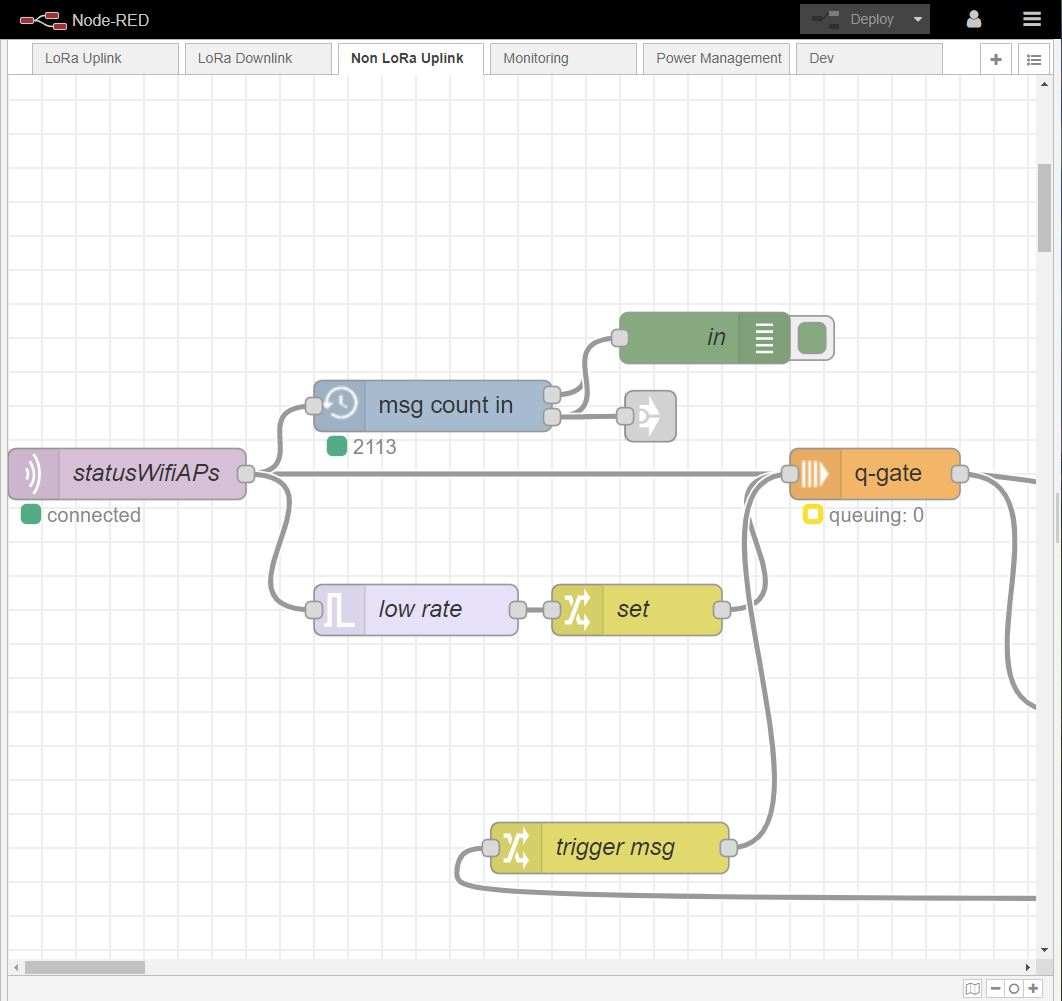
\includegraphics[width=\linewidth]{Chapters/Figures/NonLoRaUplink.JPG}}
        }
      \caption{Non LoRa Uplink Flow}
      \label{fig:Non_LoRA_Up}
    \end{figure}

\end{itemize}

\begin{itemize}
   \item \textbf{Monitoring} \\
   The Monitoring module described in figure~\ref{fig:Monitoring}, has the ability to connect with the other modules, as it is possible to observe in the left side of the figure. This module uses several counters in different check points, and combines this information to create a report. This report is then sent by e-mail to the person in charge of the model, for this work was used a daily e-mail. This module as also another function that is always analysing the different counter, and when a certain threshold is crossed, sends an SMS to the same person.\newline
 
  \begin{figure}[htbp]
  \centering
  
    {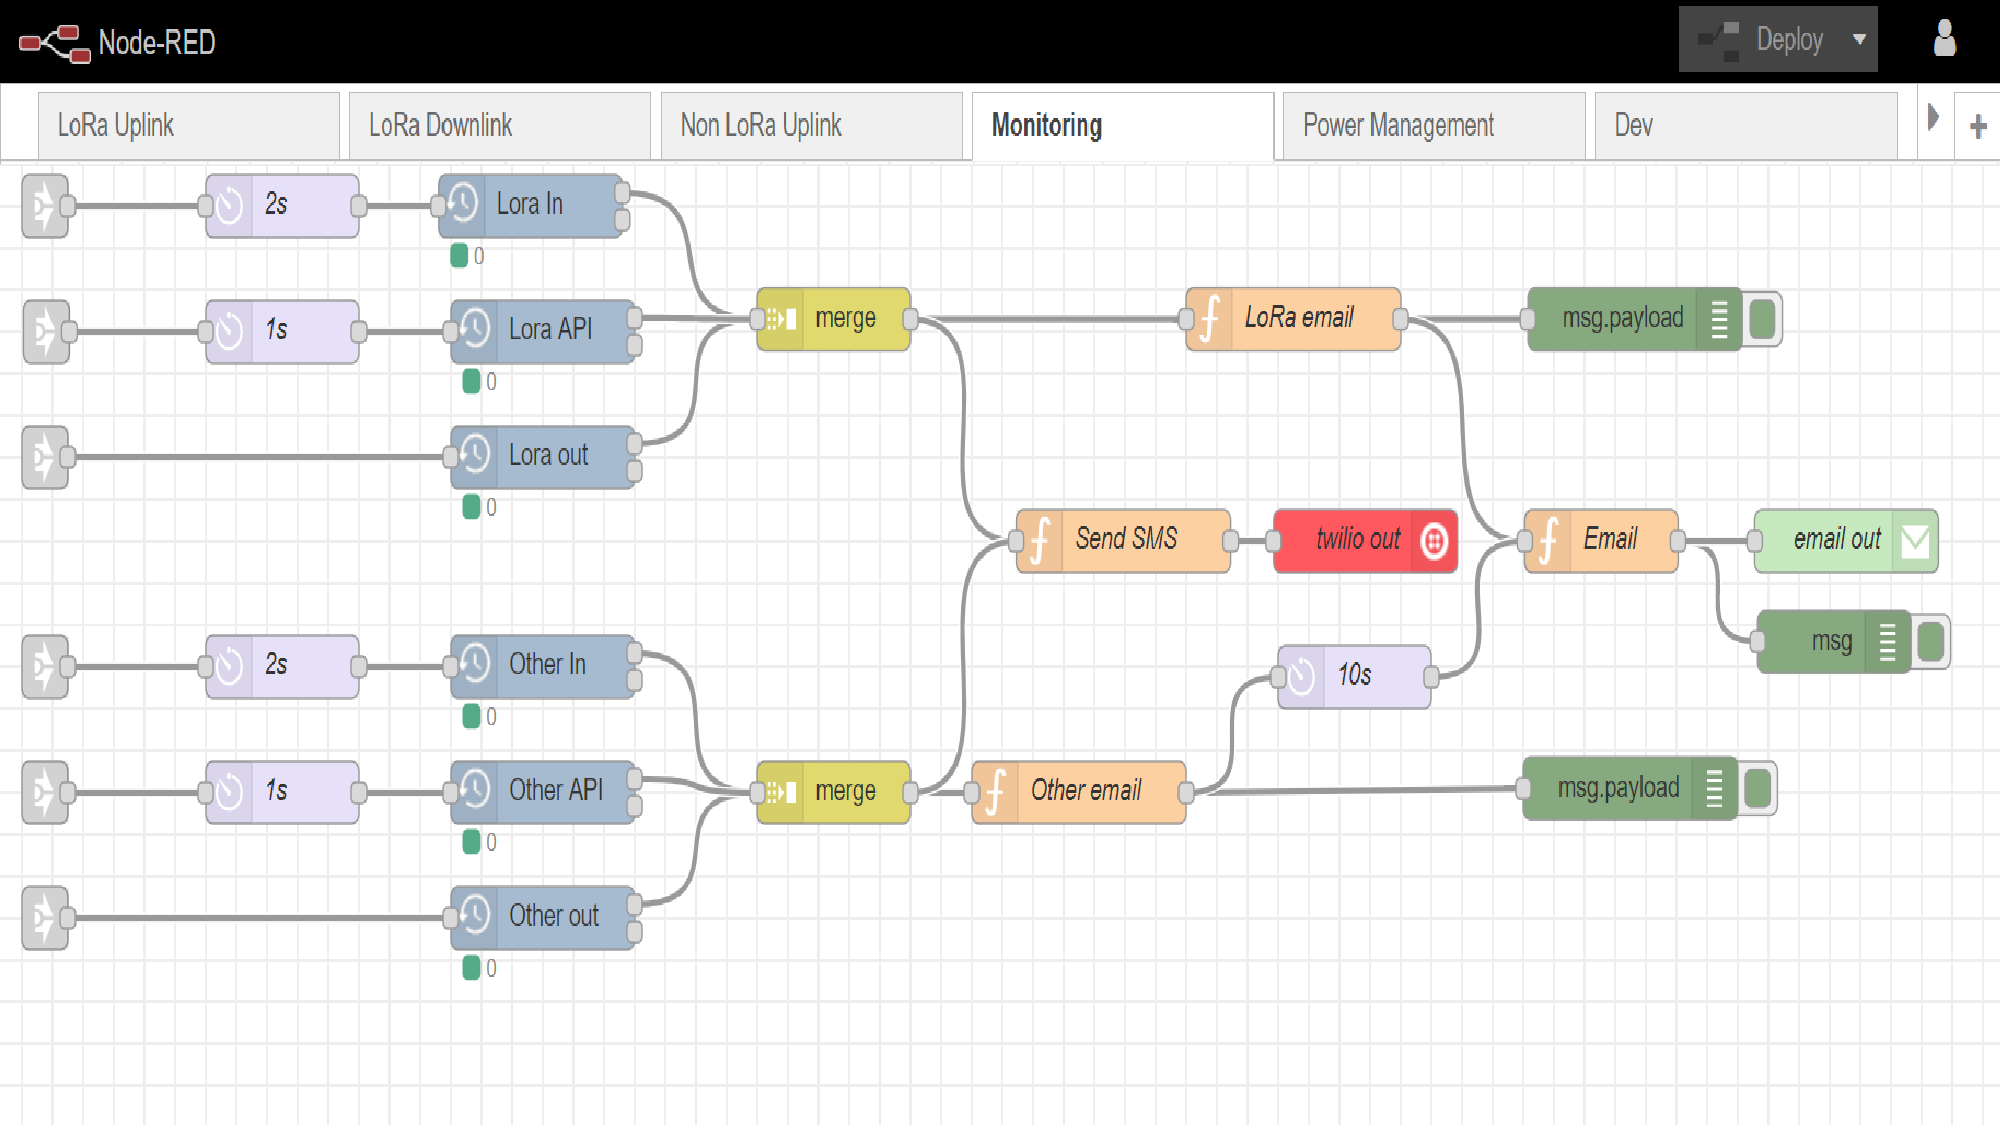
\includegraphics[width=0.9\linewidth]{Chapters/Figures/monitoring.pdf}}
 
  \caption{Monitoring Flow}
  \label{fig:Monitoring}
\end{figure}

\end{itemize}

\begin{itemize}
   \item \textbf{Security} \\
    The "Security" module is not a separated flow, but a combination of functions built in the other modules. The next figure~\ref{fig:Secu}, shows the Login Screen of the model, that requires a username and password authentication, making the "Secure Login" function. The "Drop Non-Standard Messages" is done by the first function of both uplink modules.

 \begin{figure}[htbp]
  \centering
    \scalebox{0.75}{
    {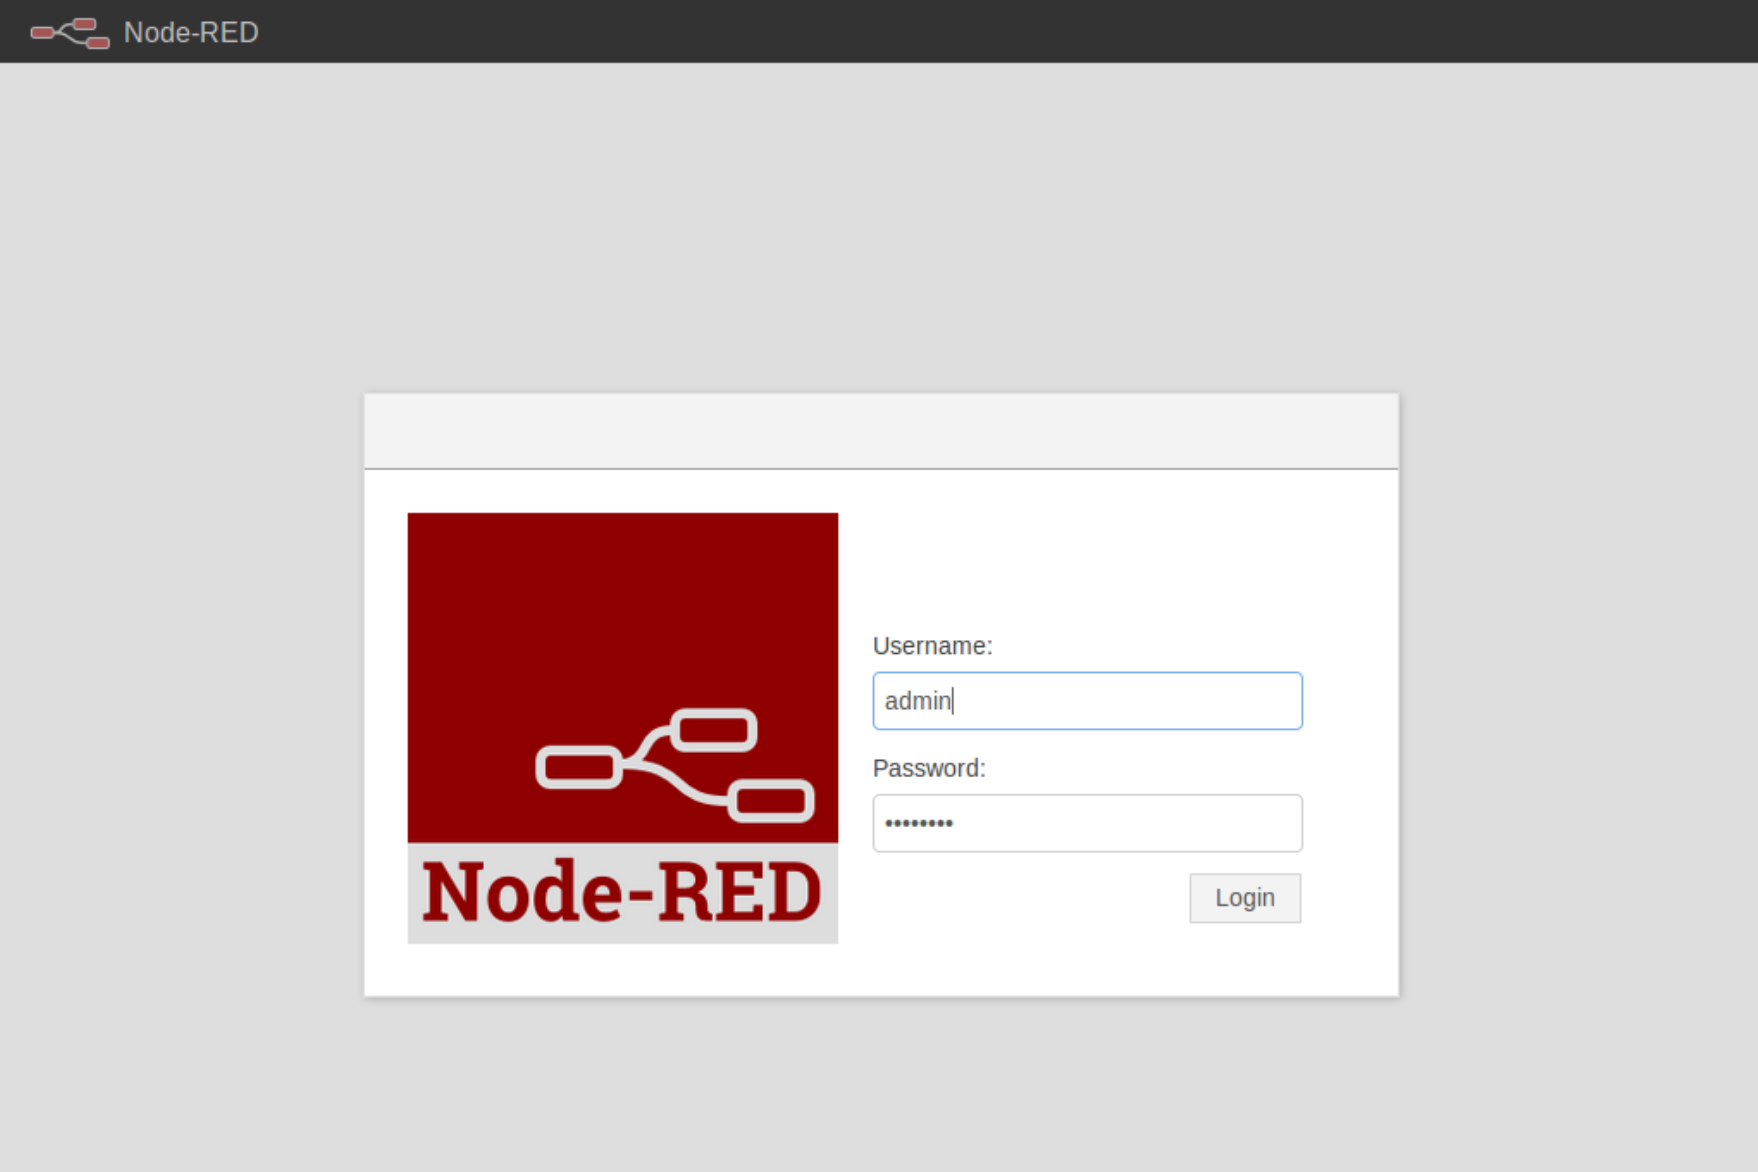
\includegraphics[width=\linewidth]{Chapters/Figures/login.PNG}}
    }
  \caption{Login Screen}
  \label{fig:Secu}
\end{figure}
\end{itemize}





% subsection nodered_sota (end)
\newpage

% section used platforms(end)
\subsection{API's }% (fold)
\label{sec:api}
An application programming interface (API) is used as an interface between the Node-Red, and the server that it is responsible for doing the calculation of the location. API's are often used as an abstraction so it is easier to use a service.

\subsubsection{Wi-Fi} % (fold)
\label{sec:wifi_sota}
The Wi-Fi~\cite{wifi} assisted location is achieved through the APIs. These APIs consume the surrounding Wi-Fi Access points and the respective~\gls{RSSI}. With this information, they do a cross-reference check in a database, and the result is sent back to the Node-Red. For this work, three APIs are used as described in chapter 5 of Appendix2~\ref{app:nodered}. The three used APIs were Google Geolocation API~\cite{GoogleLocation}, Here~\cite{Here} and OpenCellID~\cite{OpenCell}, as an alternative the Mozilla location APi~\cite{Mozilla} was also studied but at the moment of writing, there were no keys available. The next figure~\ref{fig:Google_API}, represents a test example for the Here API, using the Postman software.\newline


 
  \begin{figure}[htbp]
  \centering
  
    {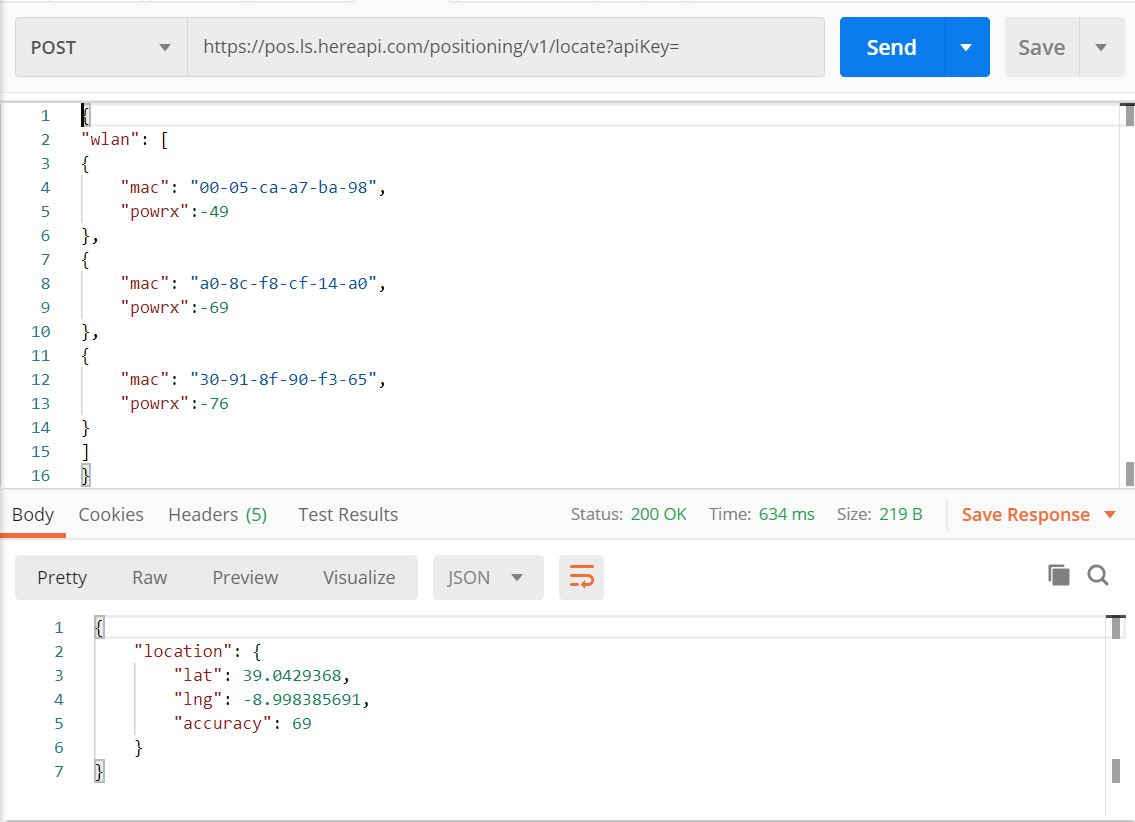
\includegraphics[width=\linewidth]{Chapters/Figures/herepost.JPG}}
 
  \caption{Here API test}
  \label{fig:Google_API}
\end{figure}








\newpage
% subsection wifi_sota (end)
\subsection{LoRa} % (fold)
\label{sec:lora_api_sota}
The LoRa~\gls{API}, used in this work, has  integration with TTN server. When the message is sent to the Node-Red server, the LoRa location is already presented in the Metadata. For this location to works, a minimum of three gateways able to listen to the transmitted message is needed.

The~\gls{API} responsible for the calculations is LoRa Cloud~\cite{LoRACloud}, former known as Collos.This~\gls{API} has three versions, all of them were used for development and testing, and the Version 2 was the one with best results, the requests made were RSSI Singleframe, TDOA Singleframe, RSSI Multiframe and TDOA Multiframe. 

The ability to use WiFi is also available but not used since there is another section for this type of assisted location. 

The~\gls{API} works in the following way: TTN receives the uplink message from one or more Gateways, and instead of throwing away duplicates, it keeps the meta-data from each one (primarily that is RSSI and SNR plus TOA if it is available).
TTN then forms a query with all the meta-data. The Query is posted to the endpoint in LoRa Cloud, specified in the configuration of the integration, and LoRa Cloud responds with a location.

TTN console then looks at the locations coming back and, if there are multiple, it sends the most accurate through~\gls{MQTT} to Node-Red.

In order to use LoRa, it was necessary to get coverage, of the local where this work was developed, for these two gateways were deployed as shown in figure~\ref{fig:LoRaGWs}, the complete guide for the instalation and configuration of the Gateways can be found at~\cite{githubnodered}.

%(Criar Imagem com pycom na caixa e fora, editar  o GW por imagem fcttopo)


\begin{figure}[htbp]
  \centering
  \subcaptionbox{Rpi with Dragino hat \label{fig:RpiLoRa}}%
    {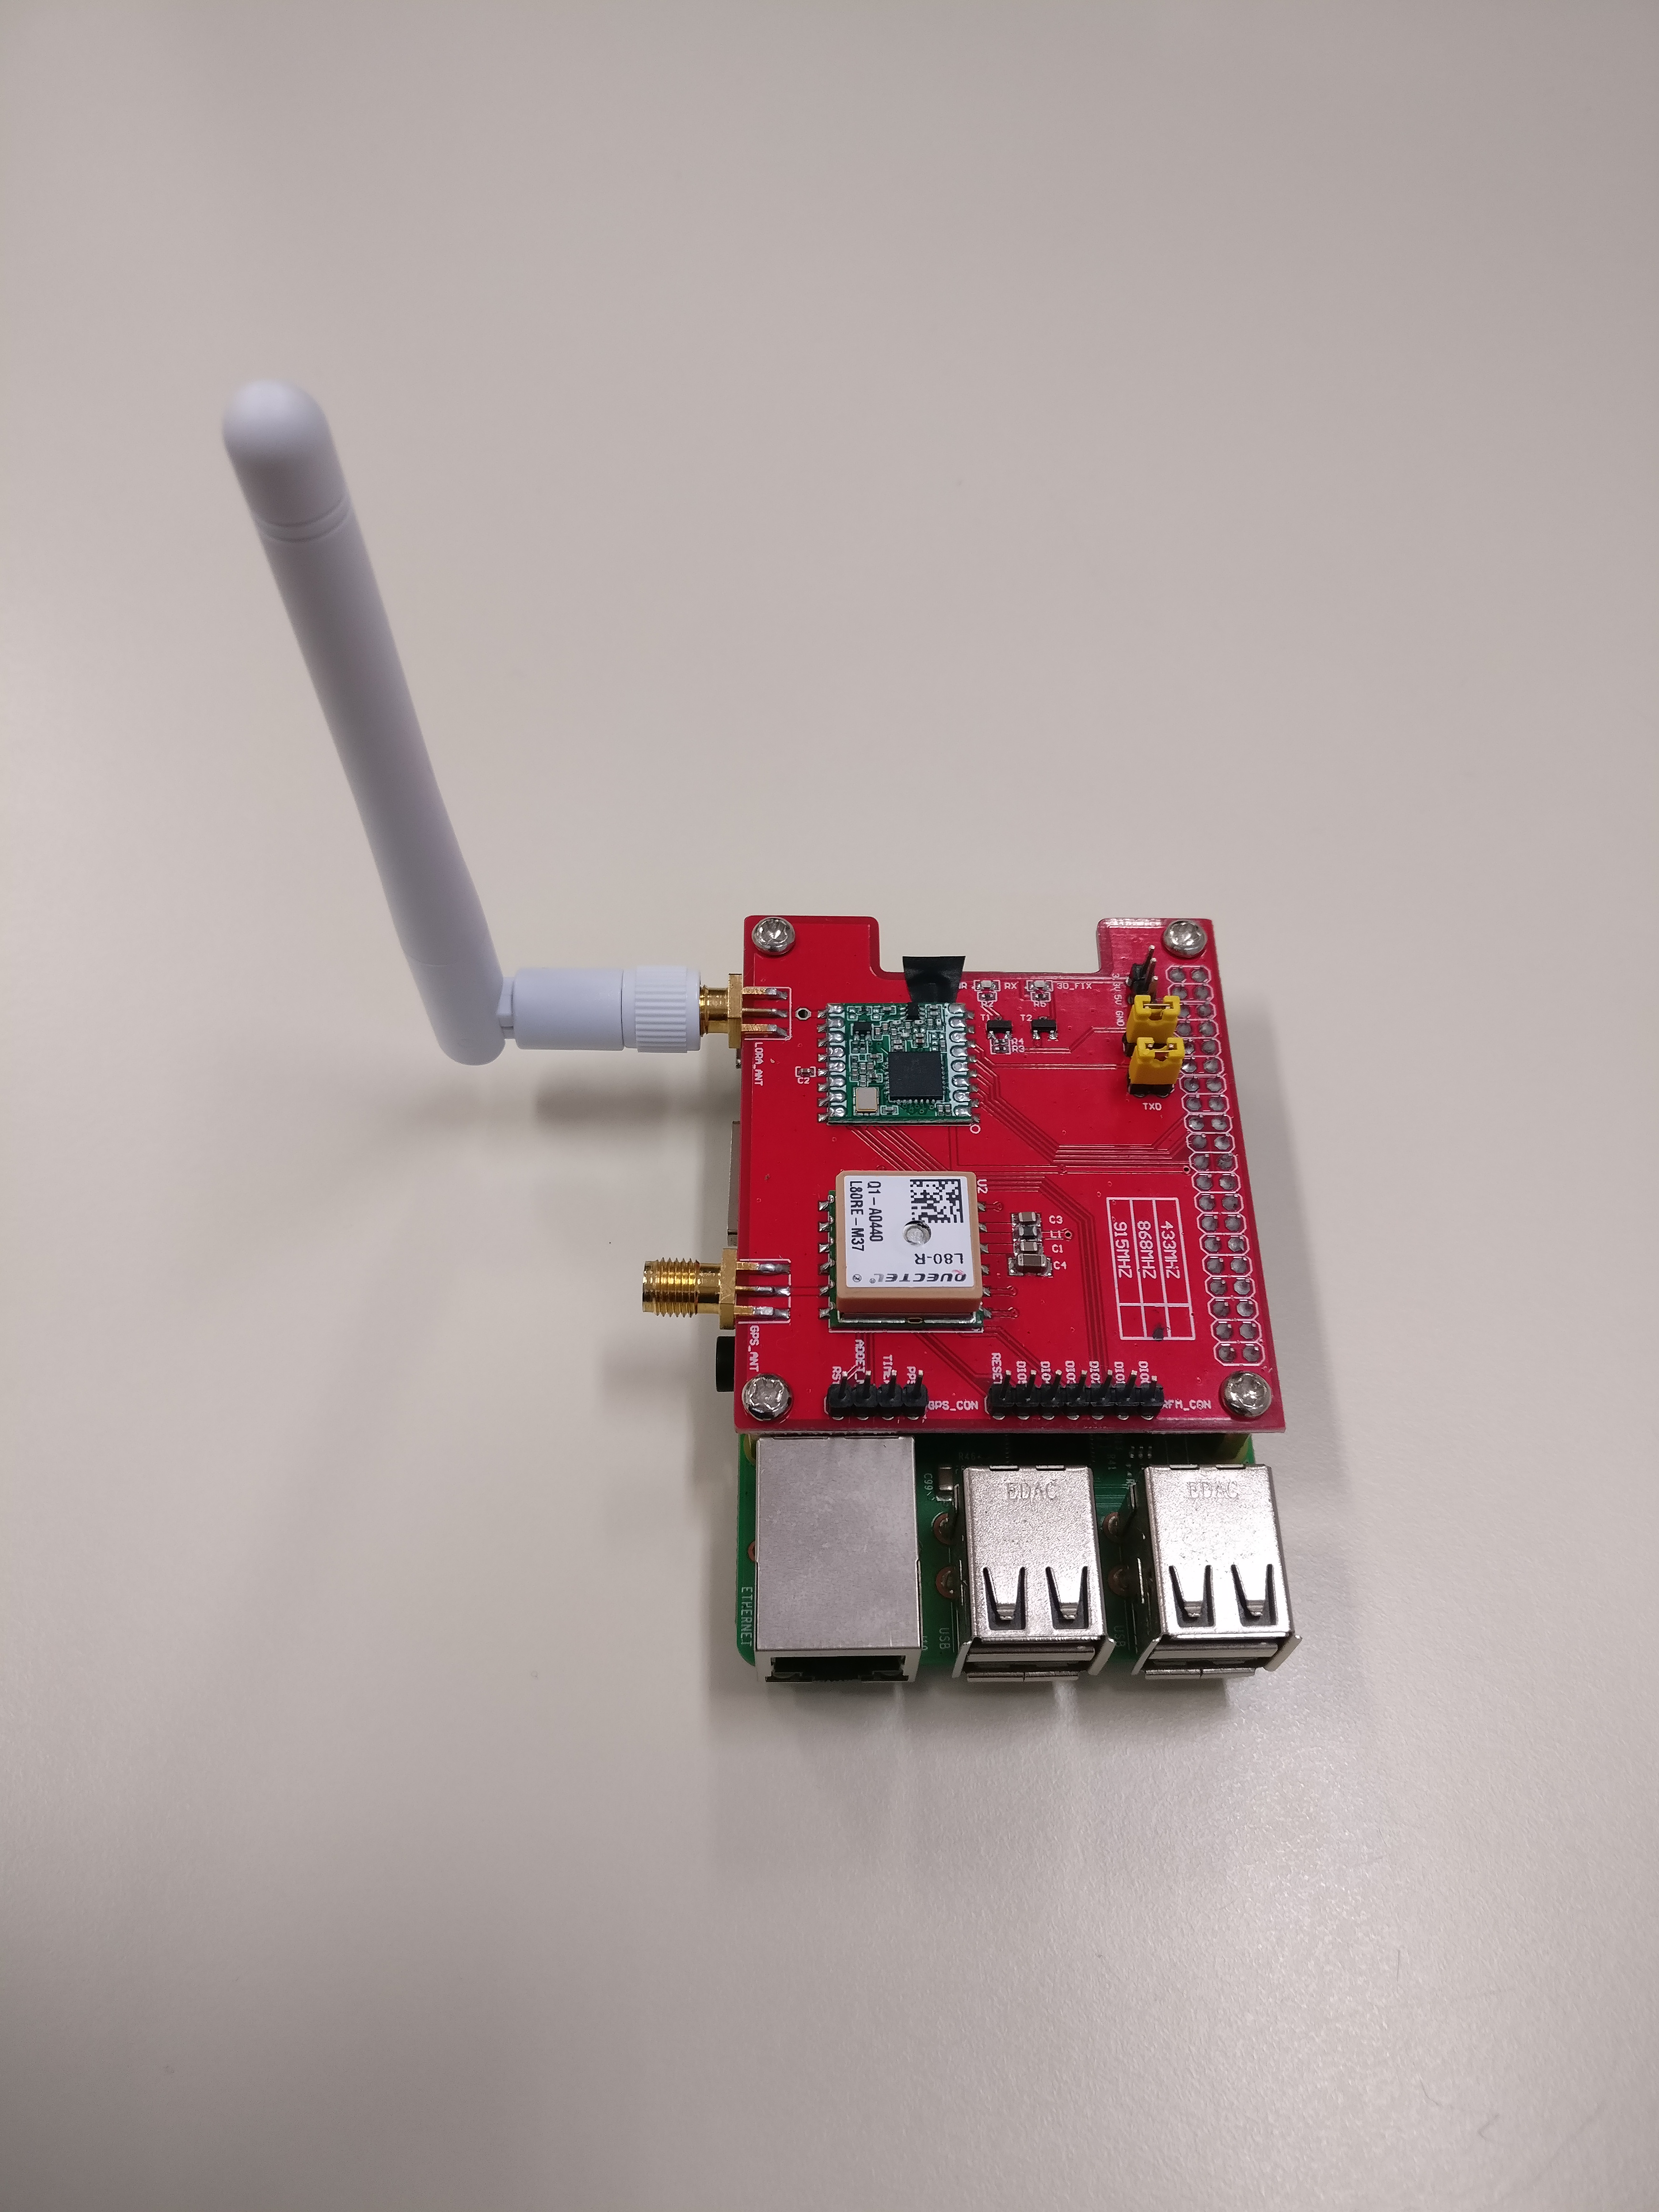
\includegraphics[height=3.5in,width=0.5\linewidth]{Chapters/Figures/rpi.jpg}}%
  \subcaptionbox{Lorix one\label{fig:Lorix}}%
    {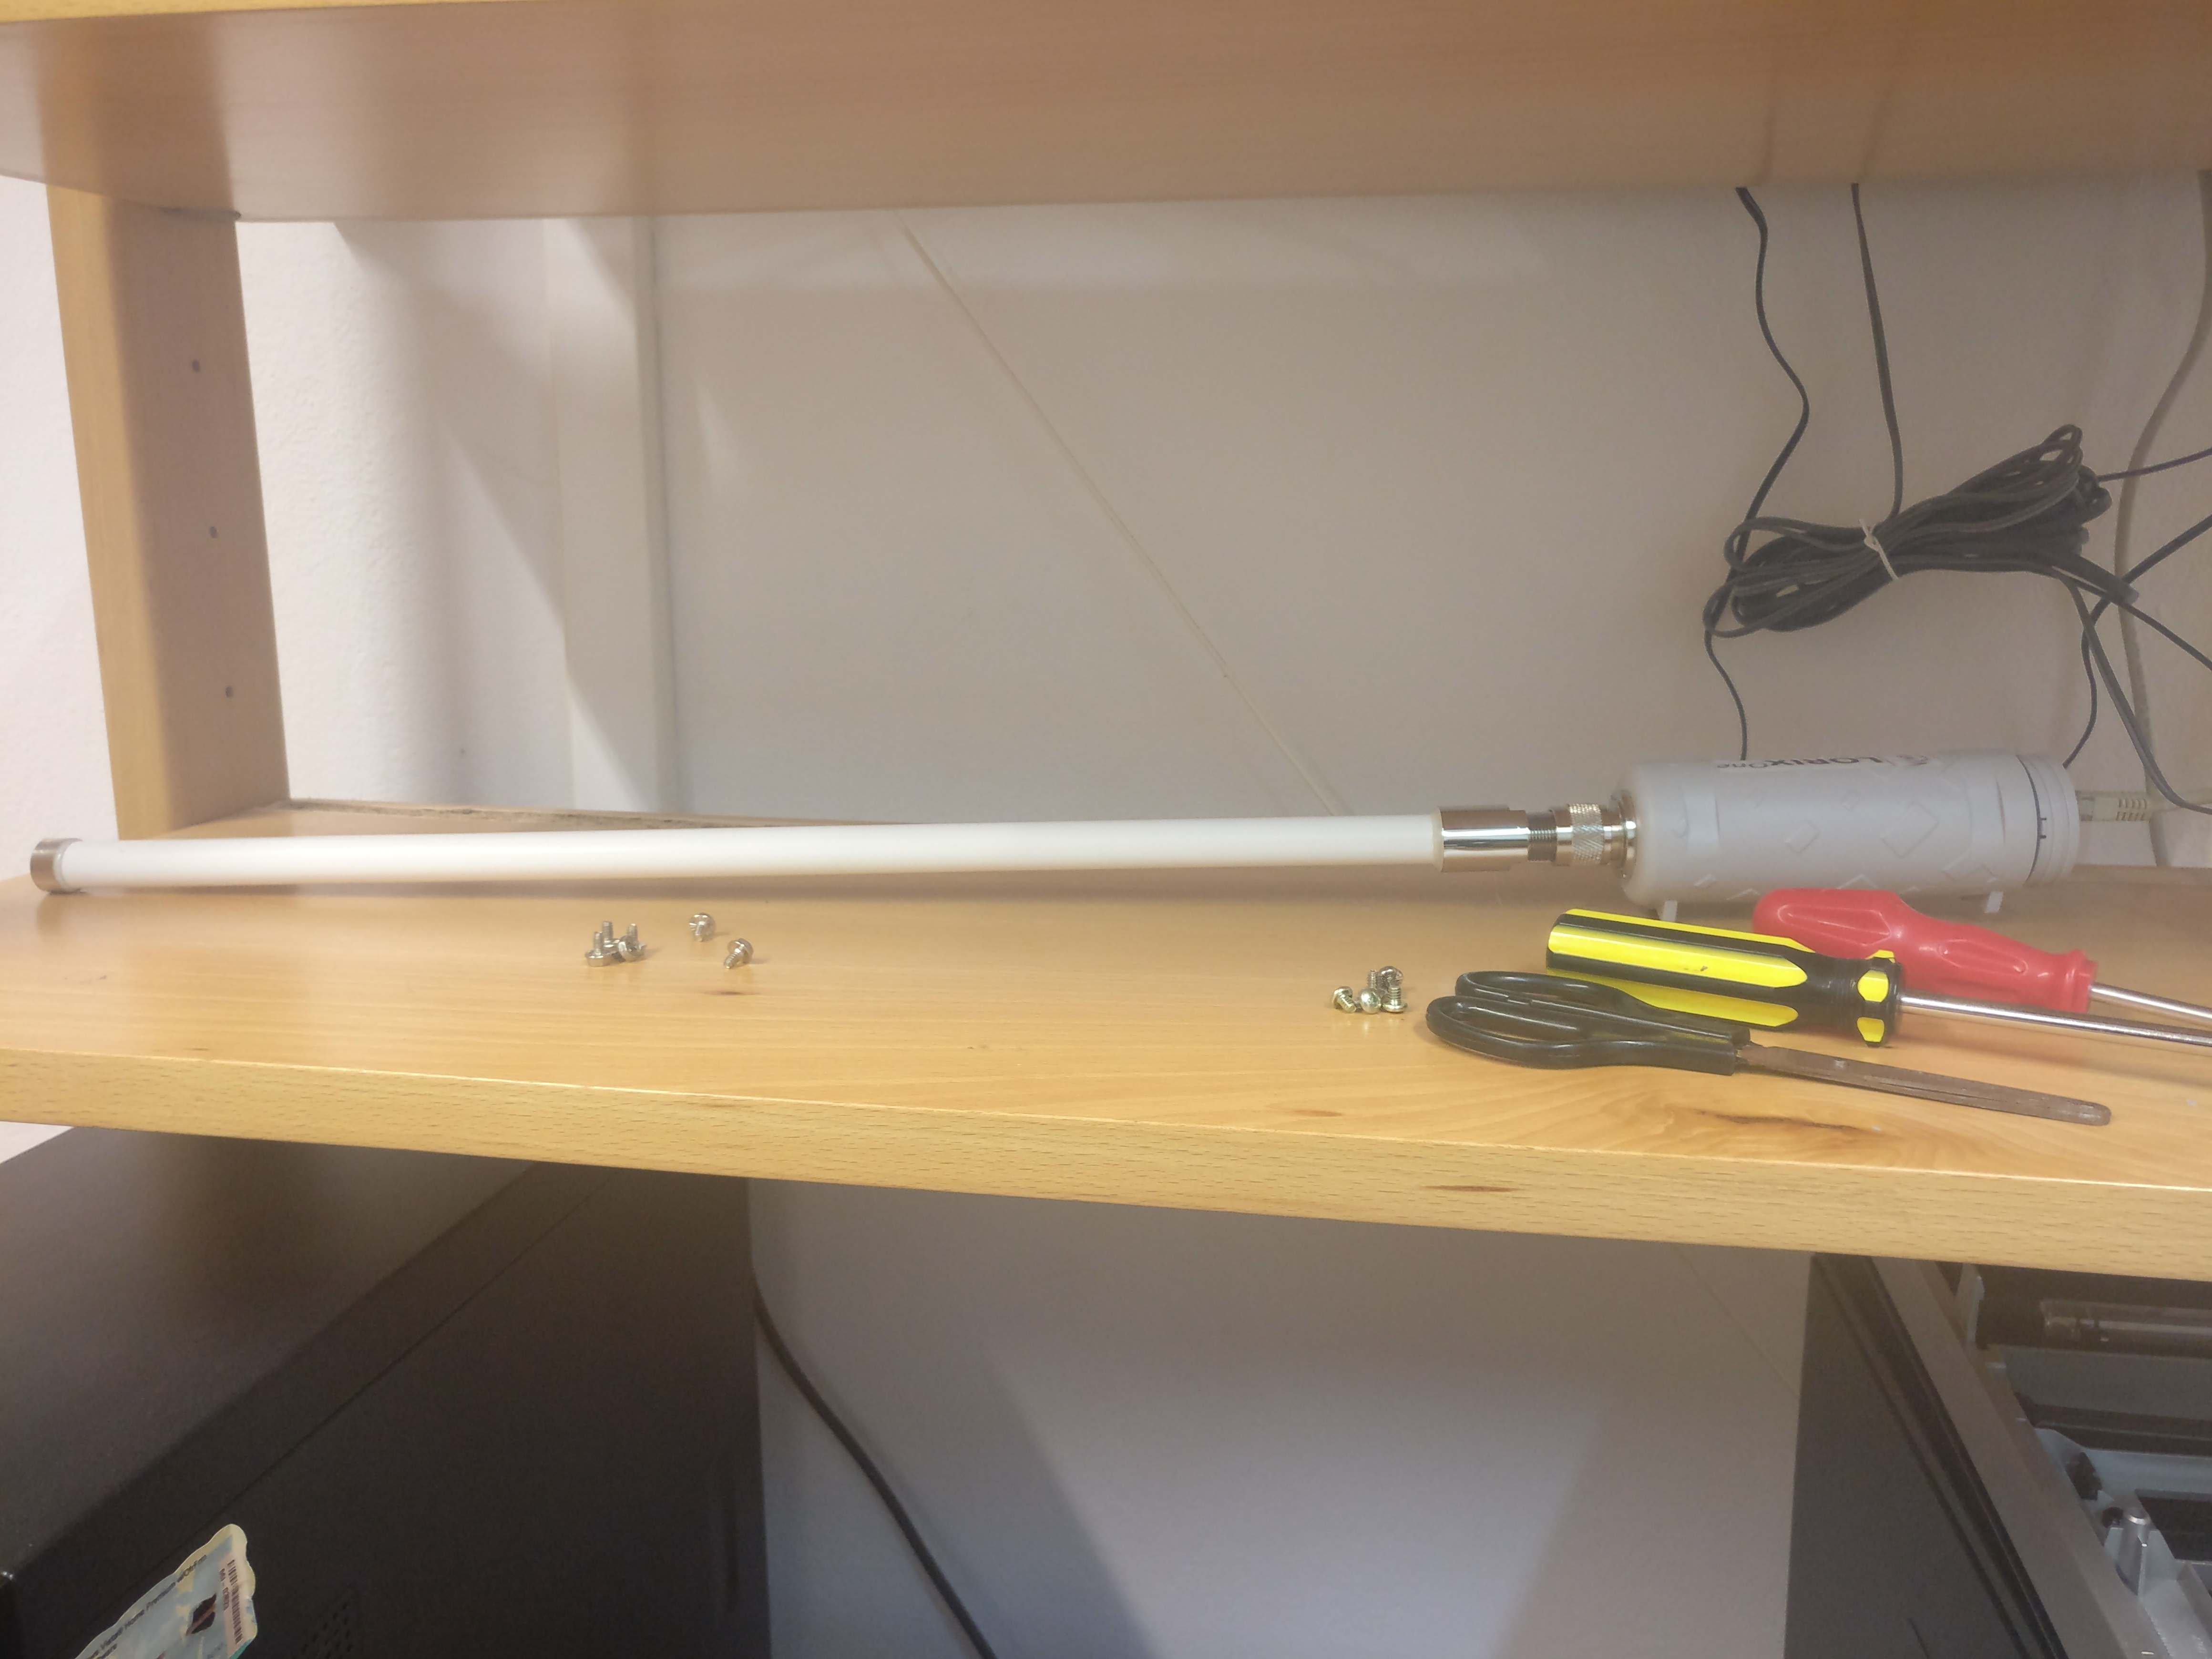
\includegraphics[height=3.5in,width=0.5\linewidth]{Chapters/Figures/Lorix.jpg}}%
  \caption{LoRa Gateways}
  \label{fig:LoRaGWs}
\end{figure}
% subsection lora_api_sota (end)
% section api's (end)




